% =============================
% GRUNDLAGEN QUANTENCOMPUTER
% =============================

\refstepcounter{chapter}
\chapter*{\thechapter. Grundlagen Quantencomputer}
\addcontentsline{toc}{chapter}{\thechapter.\space Grundlagen Quantencomputer}
Nachfolgend werden die physikalischen Grundlagen der Quantencomputertechnologie erläutert, wie Superposition, Verschränkung und Quantengatter. 
Zusätzlich werden die Unterschiede zu klassischen Computern aufgezeigt und der aktuelle Stand der Entwicklung beschrieben. 
\vspace{1em}\\
Klassische Computer speichern und verarbeiten Informationen mit Bits. Diese werden mithilfe von Transistoren realisiert
und können entweder den Wert 0 oder 1 annehmen. Gemäss dem Gesetz von Moore verdoppelt sich die Anzahl der Transistoren auf einem Chip
alle 18 bis 24 Monate, was zu einer stetigen Steigerung der Rechenleistung klassischer Computer führt \cite{mooreslaw}.
Die Rechenleistung wird gesteigert, weil die Transistoren kleiner werden. Diese sind mittlerweile nur noch drei Nanometer gross \cite{tsmc2022}. 
Da Transistoren nicht kleiner als einzelne Atome werden können, ist eine Miniaturisierung nach klassischem 
Prinzip irgendwann nicht mehr möglich \cite{mooreslaw}. Bei dieser atomaren Grössenordnung dominiert nicht mehr die klassische Physik, 
sondern die Quantenmechanik und ihre kontraintuitiven Phänomene werden zu dominanten Effekten \cite{bashiri2025quantencomputing}.
\\
Quantencomputer stellen einen grundlegend neuen Ansatz dar, indem sie die Prinzipien der 
Quantenmechanik nutzen. 
Sie arbeiten mit sogenannten Qubits (Quantenbits). 
Diese basieren auf der mikroskopischen Skala, 
wo quantenmechanische Phänomene herrschen, und nicht auf der makroskopischen Skala der klassischen Physik. 
Der entscheidende Unterschied liegt in der Natur der Qubits. 
Während klassische Bits zu jedem Zeitpunkt entweder den Zustand 0 oder 1 haben, 
können sich Qubits dank der Superposition (siehe Kapitel \ref{sec:superposition}) gleichzeitig in einer Überlagerung mehrerer Zustände befinden. 
Dies ermöglicht es Quantencomputern, Informationen auf völlig neue Art zu verarbeiten, und eröffnet das Potenzial, 
bestimmte Probleme exponentiell schneller zu lösen als klassische Computer. 
Diese exponentielle Zunahme der Rechengeschwindigkeit hat weitreichende Konsequenzen, insbesondere für die Kryptographie, 
da zahlreiche heute verwendete Verschlüsselungsverfahren durch die Rechenkapazität von Quantencomputern 
potenziell gefährdet sind \cite{bashiri2025quantencomputing}.

\pagebreak
\section{Wichtige Prinzipien der Quantenphysik}
In der Quantenphysik gibt es zwei grundlegende Prinzipien, die sie von der klassischen Physik unterscheiden und die das Verhalten von Qubits bestimmen: Superposition und Verschränkung.
\label{sec:superposition}
\subsection{Superposition}
Ein Qubit kann sich in einer Überlagerung mehrerer Zustände befinden, der sogenannten Superposition. 
Das Qubit befindet sich dabei im Zustand \hyperlink{bra-ket-def}{Ket}-Psi, dargestellt als $|\psi\rangle$.
Dieser Zustand wird ausgedrückt durch:
\begin{equation*}
|\psi\rangle = \alpha |0\rangle + \beta |1\rangle
\end{equation*}
Dabei gilt: $|\alpha|^2 + |\beta|^2 = 1$, damit die Gesamtwahrscheinlichkeit der beiden Zustände 100 \% beträgt, 
wobei $\alpha, \beta \in \mathbb{C}$.
Da $\alpha$ und $\beta$ \hyperlink{komplexe-zahlen-def}{komplexe Zahlen} sind, können sie auch als Summe von Real- und Imaginärteil dargestellt werden:
\begin{equation*}
|\psi\rangle = (Re(\alpha)+Im(\alpha)i) |0\rangle + (Re(\beta)+Im(\beta)i) |1\rangle
\end{equation*}
Dies kann auch in der polaren Schreibweise dargestellt werden:
\begin{equation*}
|\psi\rangle = r_\alpha*e^{i*\varphi_\alpha}|0\rangle + r_\beta*e^{i*\varphi_\beta}|1\rangle
\end{equation*}
$r_\alpha$ und $r_\beta$ sind die Beträge der \hyperlink{komplexe-zahlen-def}{komplexe Zahlen} $\alpha$ und $\beta$, während $\varphi_\alpha$ und $\varphi_\beta$ deren Phasenwinkel repräsentieren.
\\
Da für die Quantenmechanik nur die relative Phase zwischen den Zuständen relevant ist, wird die Phase $\varphi_\alpha$ auf 0° gesetzt und $\varphi_\beta = \varphi_\beta - \varphi_\alpha$.
Die folgenden Abbildungen in Tabelle \ref{tab:bilder_ueberblick} zeigen den Unterschied zwischen Amplituden- und Phasenanteilen eines Qubits.
\vspace{5pt}
\begin{table}[ht]
    \centering
    \caption{Überblick Amplituden- und Phasenanteile eines Qubits}
    \label{tab:bilder_ueberblick}
    \small
    \begin{tabular}{|c|c|}
        \hline
    \begin{minipage}[c]{0.35\linewidth}
    \centering
    \vspace{10pt}
    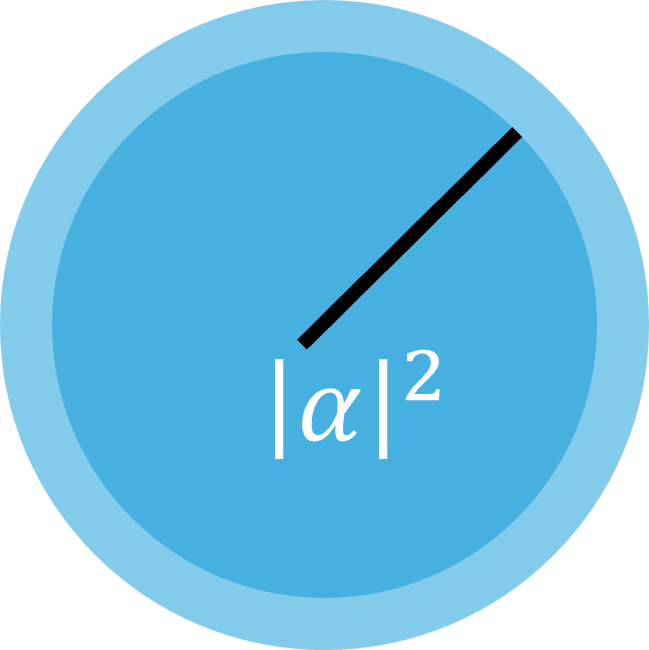
\includegraphics[width=0.4\linewidth]{images/phase_alpha_1.png}\\
    \vspace{4pt}
    \footnotesize $|\alpha|^2 = 0.7 \rightarrow$
    $70 \; \%$ Wahrscheinlichkeit für Zustand 0\\
    Phase $\varphi_\alpha = 45^\circ$\\
    \vspace{10pt}
    \end{minipage}
    &
    \begin{minipage}[c]{0.35\linewidth}
    \centering
    \vspace{10pt}
    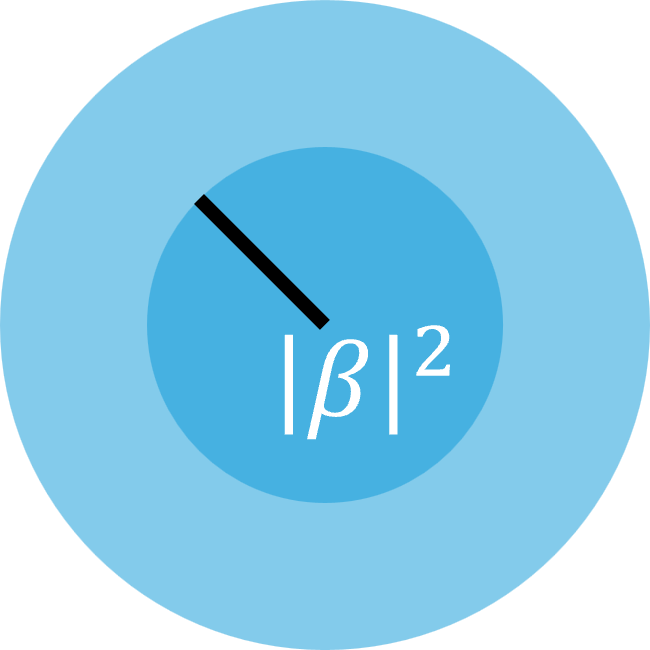
\includegraphics[width=0.4\linewidth]{images/phase_beta_1.png}\\
    \vspace{4pt}
    \footnotesize $|\beta|^2 = 0.3 \rightarrow$
    $30 \; \%$ Wahrscheinlichkeit für Zustand 1\\
    Phase $\varphi_\beta = 135^\circ$\\
    \vspace{10pt}
    \end{minipage}
    \\
    \hline
    \begin{minipage}[c]{0.35\linewidth}
    \centering
    \vspace{10pt}
    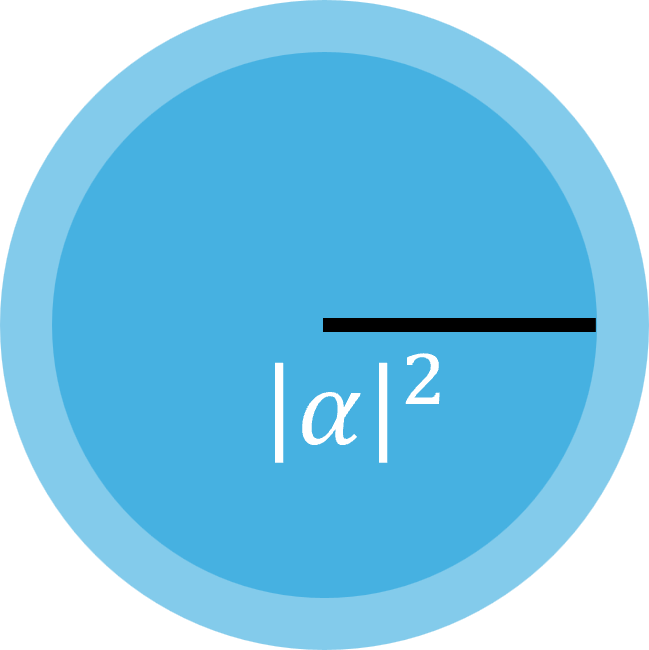
\includegraphics[width=0.4\linewidth]{images/phase_alpha_2.png}\\
    \vspace{4pt}
    \footnotesize $|\alpha|^2 = 0.7 \rightarrow$
    $70 \; \%$ Wahrscheinlichkeit für Zustand 0\\
    Phase $\varphi_\alpha = 0^\circ$\\
    \vspace{10pt}
    \end{minipage}
    &
    \begin{minipage}[c]{0.35\linewidth}
    \centering
    \vspace{10pt}
    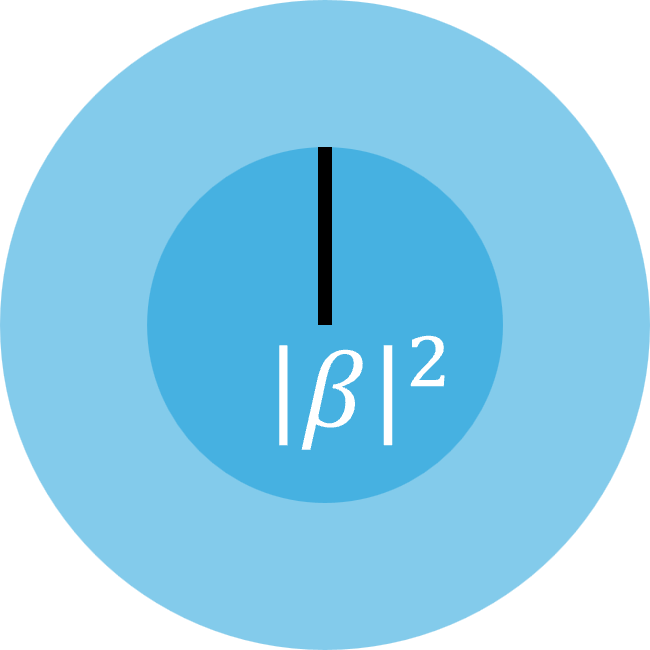
\includegraphics[width=0.4\linewidth]{images/phase_beta_2.png}\\
    \vspace{4pt}
    \footnotesize $|\beta|^2 = 0.3 \rightarrow$
    $30 \; \%$ Wahrscheinlichkeit für Zustand 1\\
    Phase $\varphi_\beta = 135^\circ - 45^\circ = 90^\circ$\\
    \vspace{10pt}
    \end{minipage}
    \\
    \hline
    \end{tabular}
\end{table}
\vspace{5pt}
\\
Um nur die relative Phase zu berücksichtigen, werden beide Seiten der Gleichung mit dem Faktor $e^{-i*\varphi_\alpha}$ multipliziert:
\begin{equation*}
|\psi\rangle \equiv r_\alpha|0\rangle + r_\beta*e^{i*(\varphi_\beta - \varphi_\alpha)}|1\rangle
\end{equation*}
\\
$\varphi$ wird definiert als $\varphi_\beta - \varphi_\alpha$\\
$\varphi \in \mathbb{R} [0, 2\pi]$\\
Somit ergibt sich die vereinfachte Darstellung \cite{youtube2024quantencomputing}:
\begin{equation*}
|\psi\rangle = r_\alpha|0\rangle + r_\beta*e^{i*(\varphi)}|1\rangle
\end{equation*}
Da $r_\alpha$ und $r_\beta$ die Beträge der \hyperlink{komplexe-zahlen-def}{komplexe Zahlen} $\alpha$ und $\beta$ sind, gilt weiterhin: $r_\alpha^2 + r_\beta^2 = 1$.
Dadurch lassen sich $r_\alpha$ und $r_\beta$ als Längen in einem Einheitskreis darstellen (siehe Abbildung \ref{fig:einheitskreis_trigonometrie}) \cite{youtube2020blochkugel}.
\begin{figure}[ht]
    \centering
    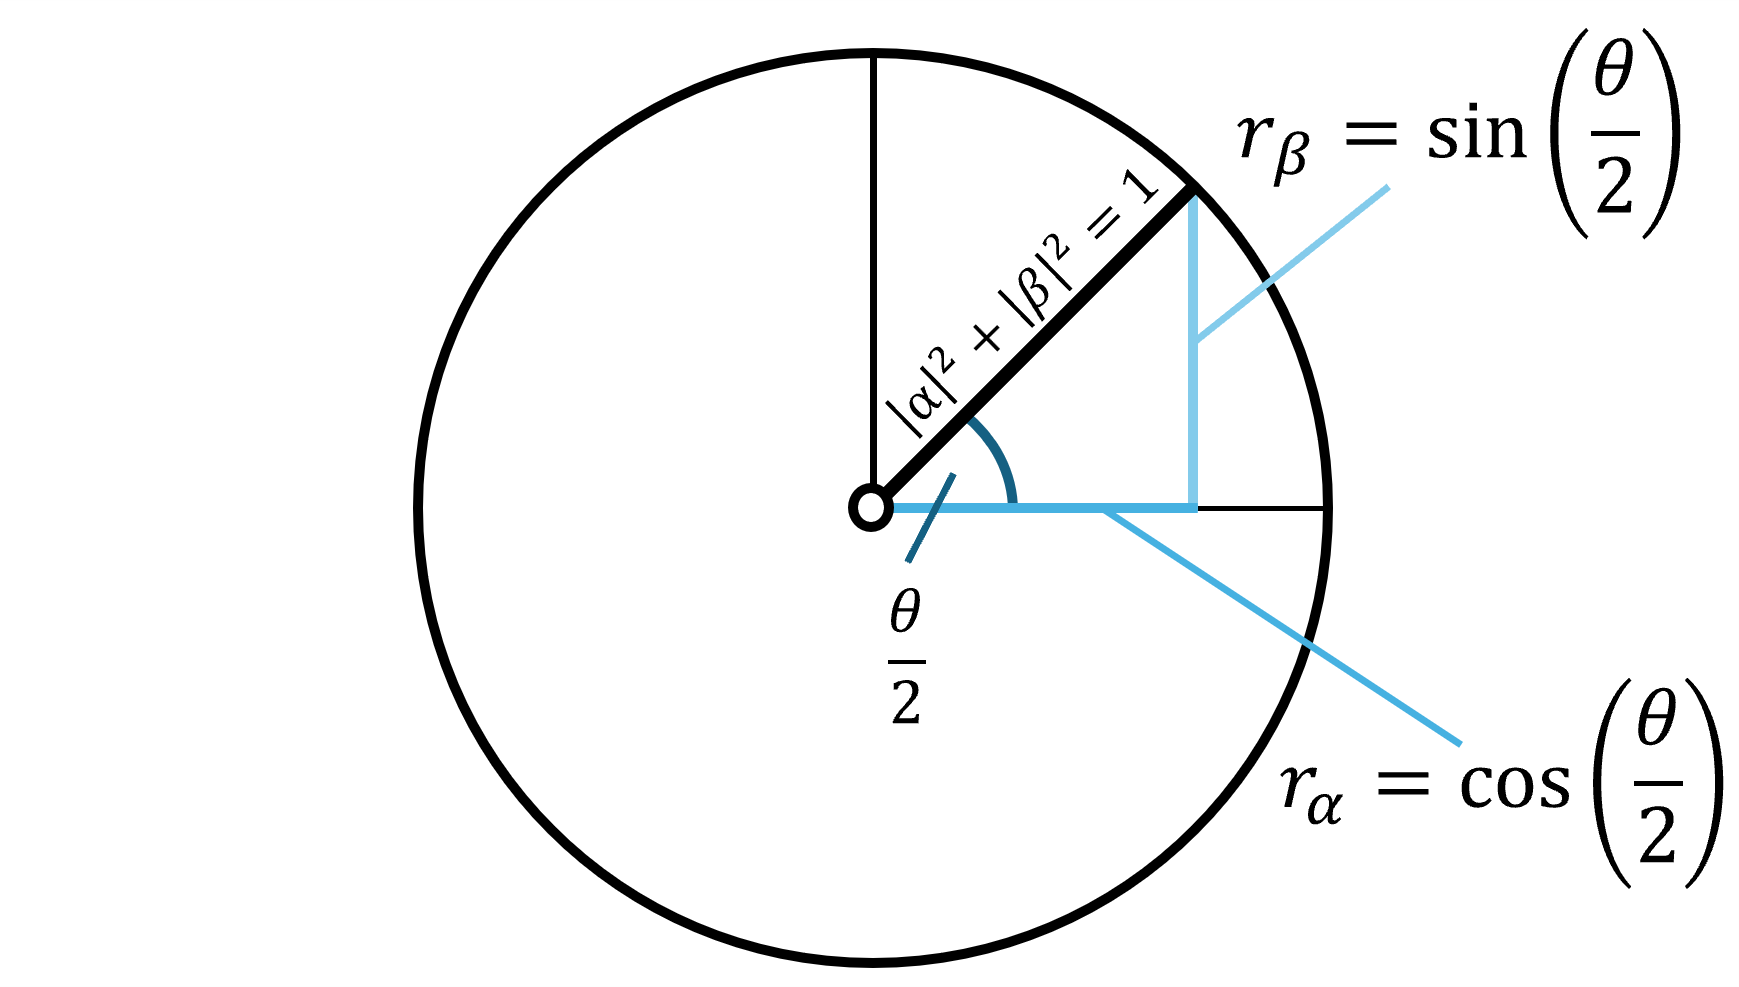
\includegraphics[height=0.25\linewidth]{images/trigonometric_visualization_alpha_beta.png}
    \caption{Trigonometrische Visualisierung von $r_\alpha$ und $r_\beta$}
    \label{fig:einheitskreis_trigonometrie}
    %eigene darstellung
\end{figure}
\\
$\theta \in \mathbb{R} \left[0, \pi\right]$ ist der Winkel im Einheitskreis, welcher sich aus dem Verhältnis von $r_\alpha$ und $r_\beta$ ergibt.
Somit gilt: $r_\alpha = cos(\frac{\theta}{2})$ und $r_\beta = sin(\frac{\theta}{2})$\\
\\
Mit Hilfe der Trigonometrie lässt sich dies auch wie folgt darstellen:\\
\begin{equation*}
    |\psi\rangle = cos(\frac{\theta}{2})|0\rangle + sin(\frac{\theta}{2})*e^{i*\varphi}|1\rangle
\end{equation*}
Wobei $\theta$ der Winkel zwischen dem Zustand $|0\rangle$ und dem Zustand $|\psi\rangle$ ist.
Dies lässt sich, wie unten skizziert auch auf der Bloch-Kugel visualisieren \cite{youtube2024quantencomputing}.
\begin{figure}[ht]
    \centering
    \includegraphics[height=0.35\linewidth]{images/bloch_sphere.png}
    \caption{Bloch-Kugel \cite{wiki2024blochsphere}}
    \label{fig:bloch_kugel}
\end{figure}

\newpage
\subsection{Verschränkung}
Ein weiteres Prinzip der Quantenphysik ist die Verschränkung.
Sind zwei Qubits verschränkt, ist der Zustand des einen Qubits untrennbar mit dem Zustand des anderen verbunden.
Durch die Messung eines Qubits entscheidet sich dieses für einen eindeutigen binären Zustand (0 oder 1) und die Superposition kollabiert. 
Die Wahrscheinlichkeit für den Zustand 0 beträgt $|\alpha|^2$ und für den Zustand 1 beträgt sie $|\beta|^2$.
Das andere Qubit nimmt sofort den korrespondierenden Zustand an, unabhängig von der Entfernung zwischen den beiden Qubits. 
Warum dies so ist, ist bis heute nicht vollständig geklärt \cite{bashiri2025quantencomputing}.

\section{Quantengatter}
Quantencomputer können im Gegensatz zu klassischen Computern keine Variablen deklarieren und Funktionen oder Schleifen erstellen.
Stattdessen werden die Qubits durch Quantengatter manipuliert analog zu logischen Gattern in klassischen Computern \cite{ct2020quantengatter}.
Wie bei \hyperlink{fpga-def}{Field-Programmable Gate Array-Schaltungen} (FPGA-Schaltungen) werden die Qubits durch eine Abfolge von Quantengattern geführt, um Berechnungen durchzuführen.
Bei klassischen Computern sind nicht alle Gatter invertierbar, d.h., bei einem \hyperlink{xor-gate-def}{XOR-Gatter} lässt sich anhand des Ausgangs nicht bestimmen,
welche Bits am Eingang anliegen. Bei Quantencomputern hingegen sind alle Quantengatter invertierbar \cite{ct2022quantencomputer}.
\\
Nachfolgend sind die wichtigsten Quantengatter aufgeführt:
\begin{itemize}
    \item Pauli-Gatter (X, Y, Z): Ein Pauli-Gatter dreht den Zustand eines Qubits um die x-, y- oder z-Achse der Bloch-Kugel \cite{bashiri2025quantencomputing}.
    
    \begin{table}[ht]
        \centering
        \caption{Pauli-Gatter Darstellung}
        \label{tab:pauli_gates}
        \begin{tabular}{|c|c|c|}
            \hline
            \raisebox{-.5\height}{\parbox[c]{1em}{\centering X}} & \raisebox{-.5\height}{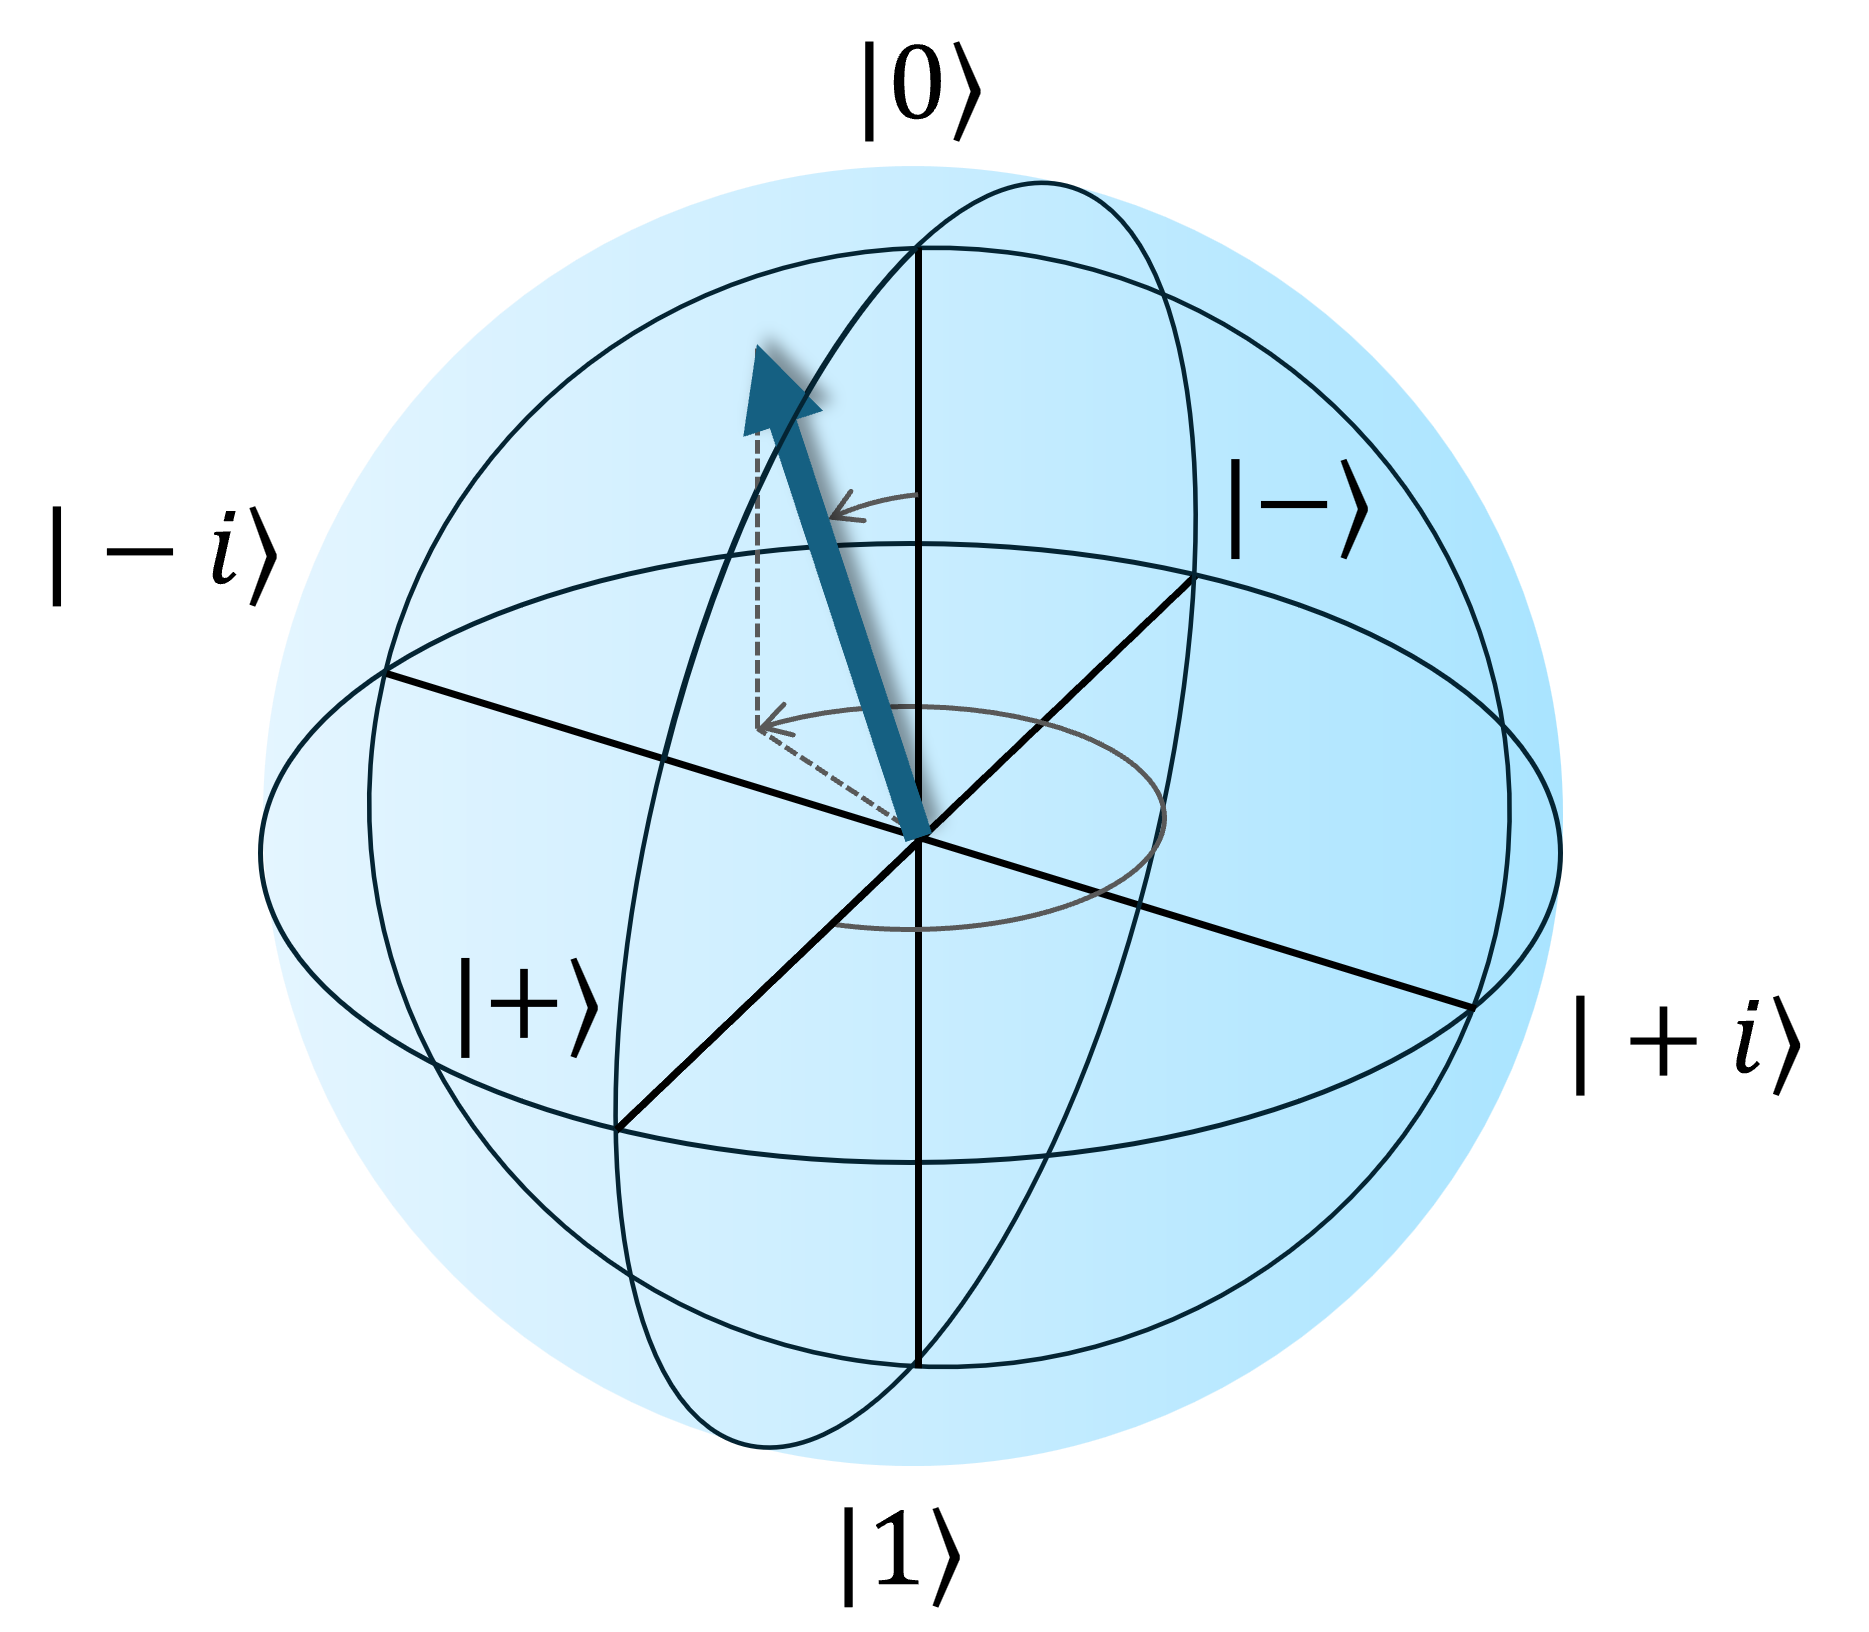
\includegraphics[width=0.22\linewidth]{images/PauliX_gate0.png}} &
            \raisebox{-.5\height}{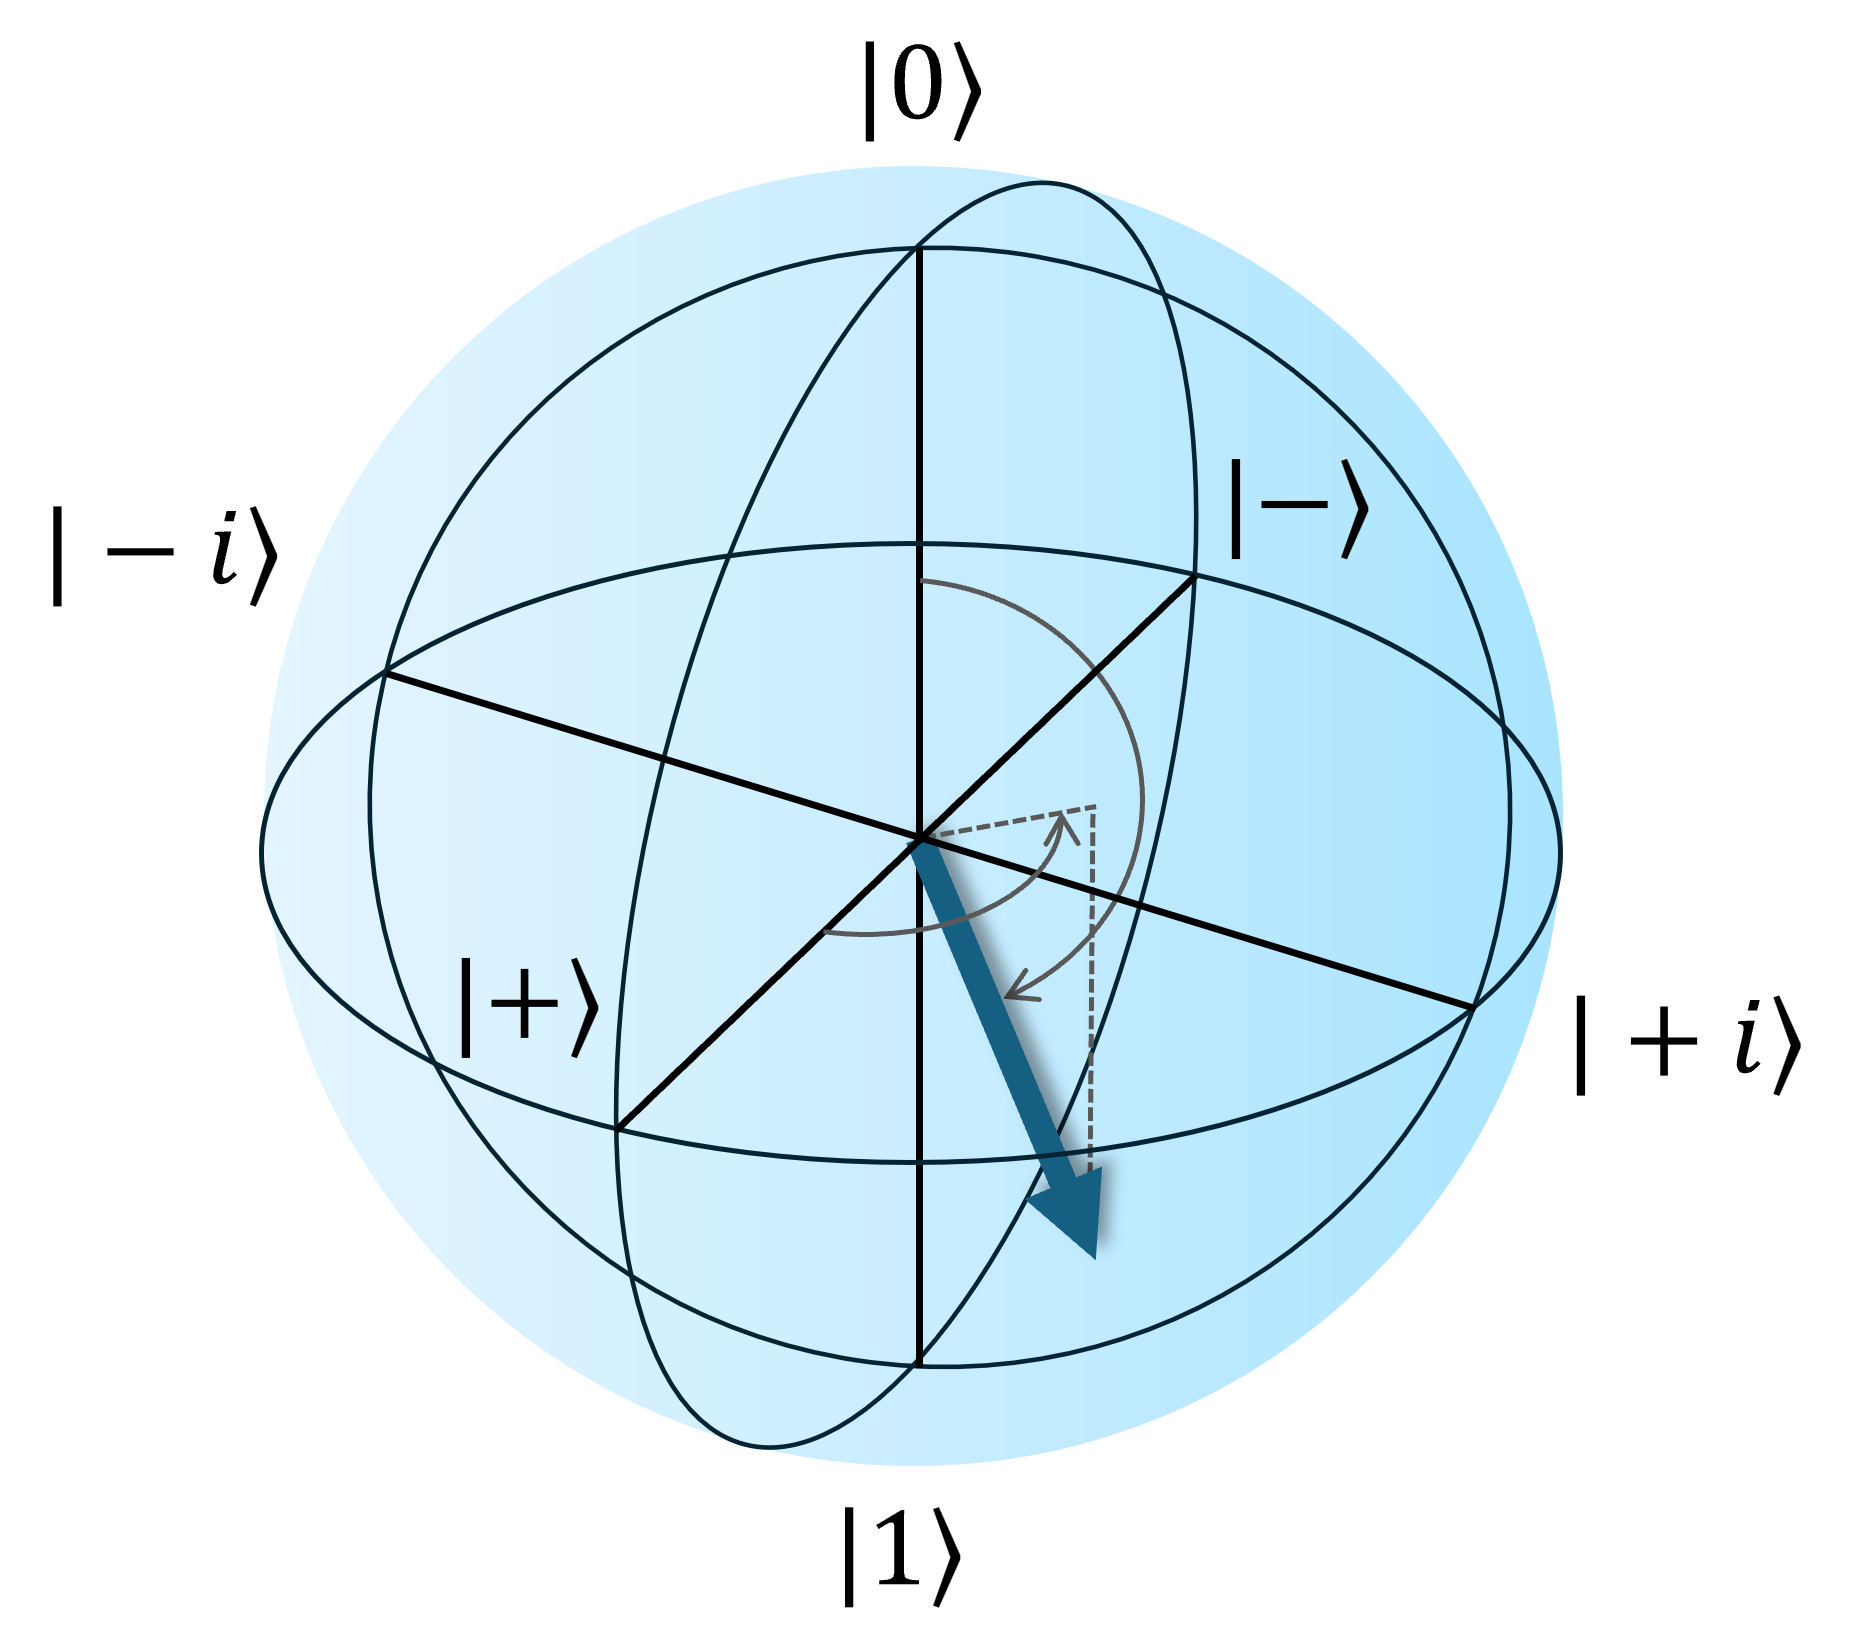
\includegraphics[width=0.22\linewidth]{images/PauliX_gate1.png}} \\[10pt]
            \hline
            \raisebox{-.5\height}{\parbox[c]{1em}{\centering Y}} & \raisebox{-.5\height}{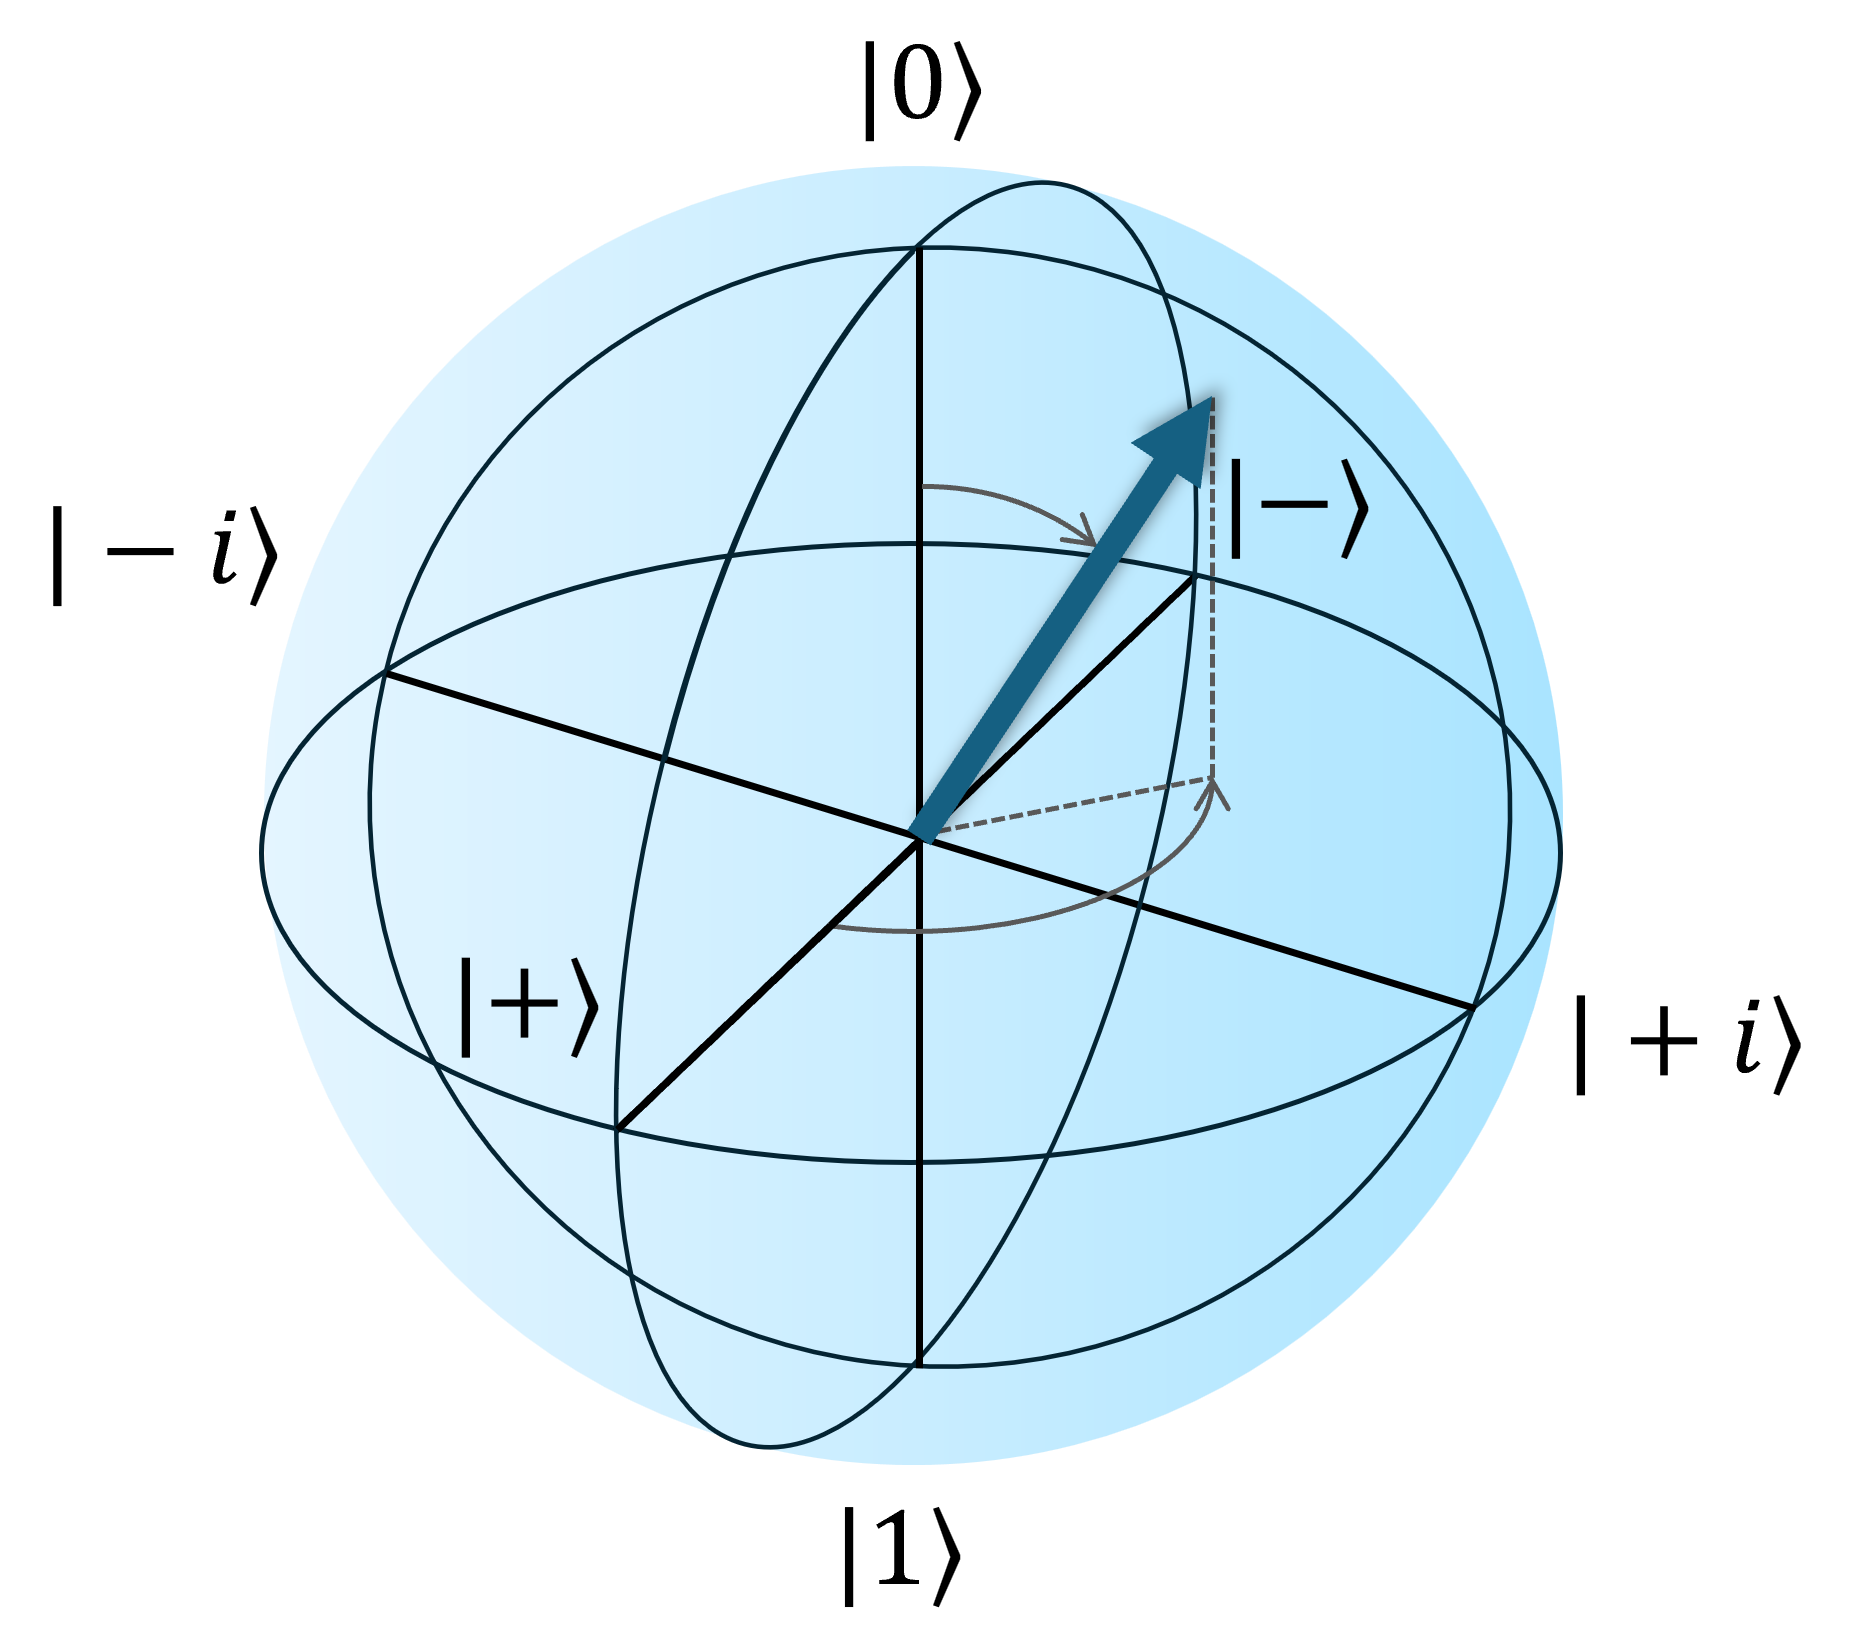
\includegraphics[width=0.22\linewidth]{images/PauliY_gate0.png}} &
            \raisebox{-.5\height}{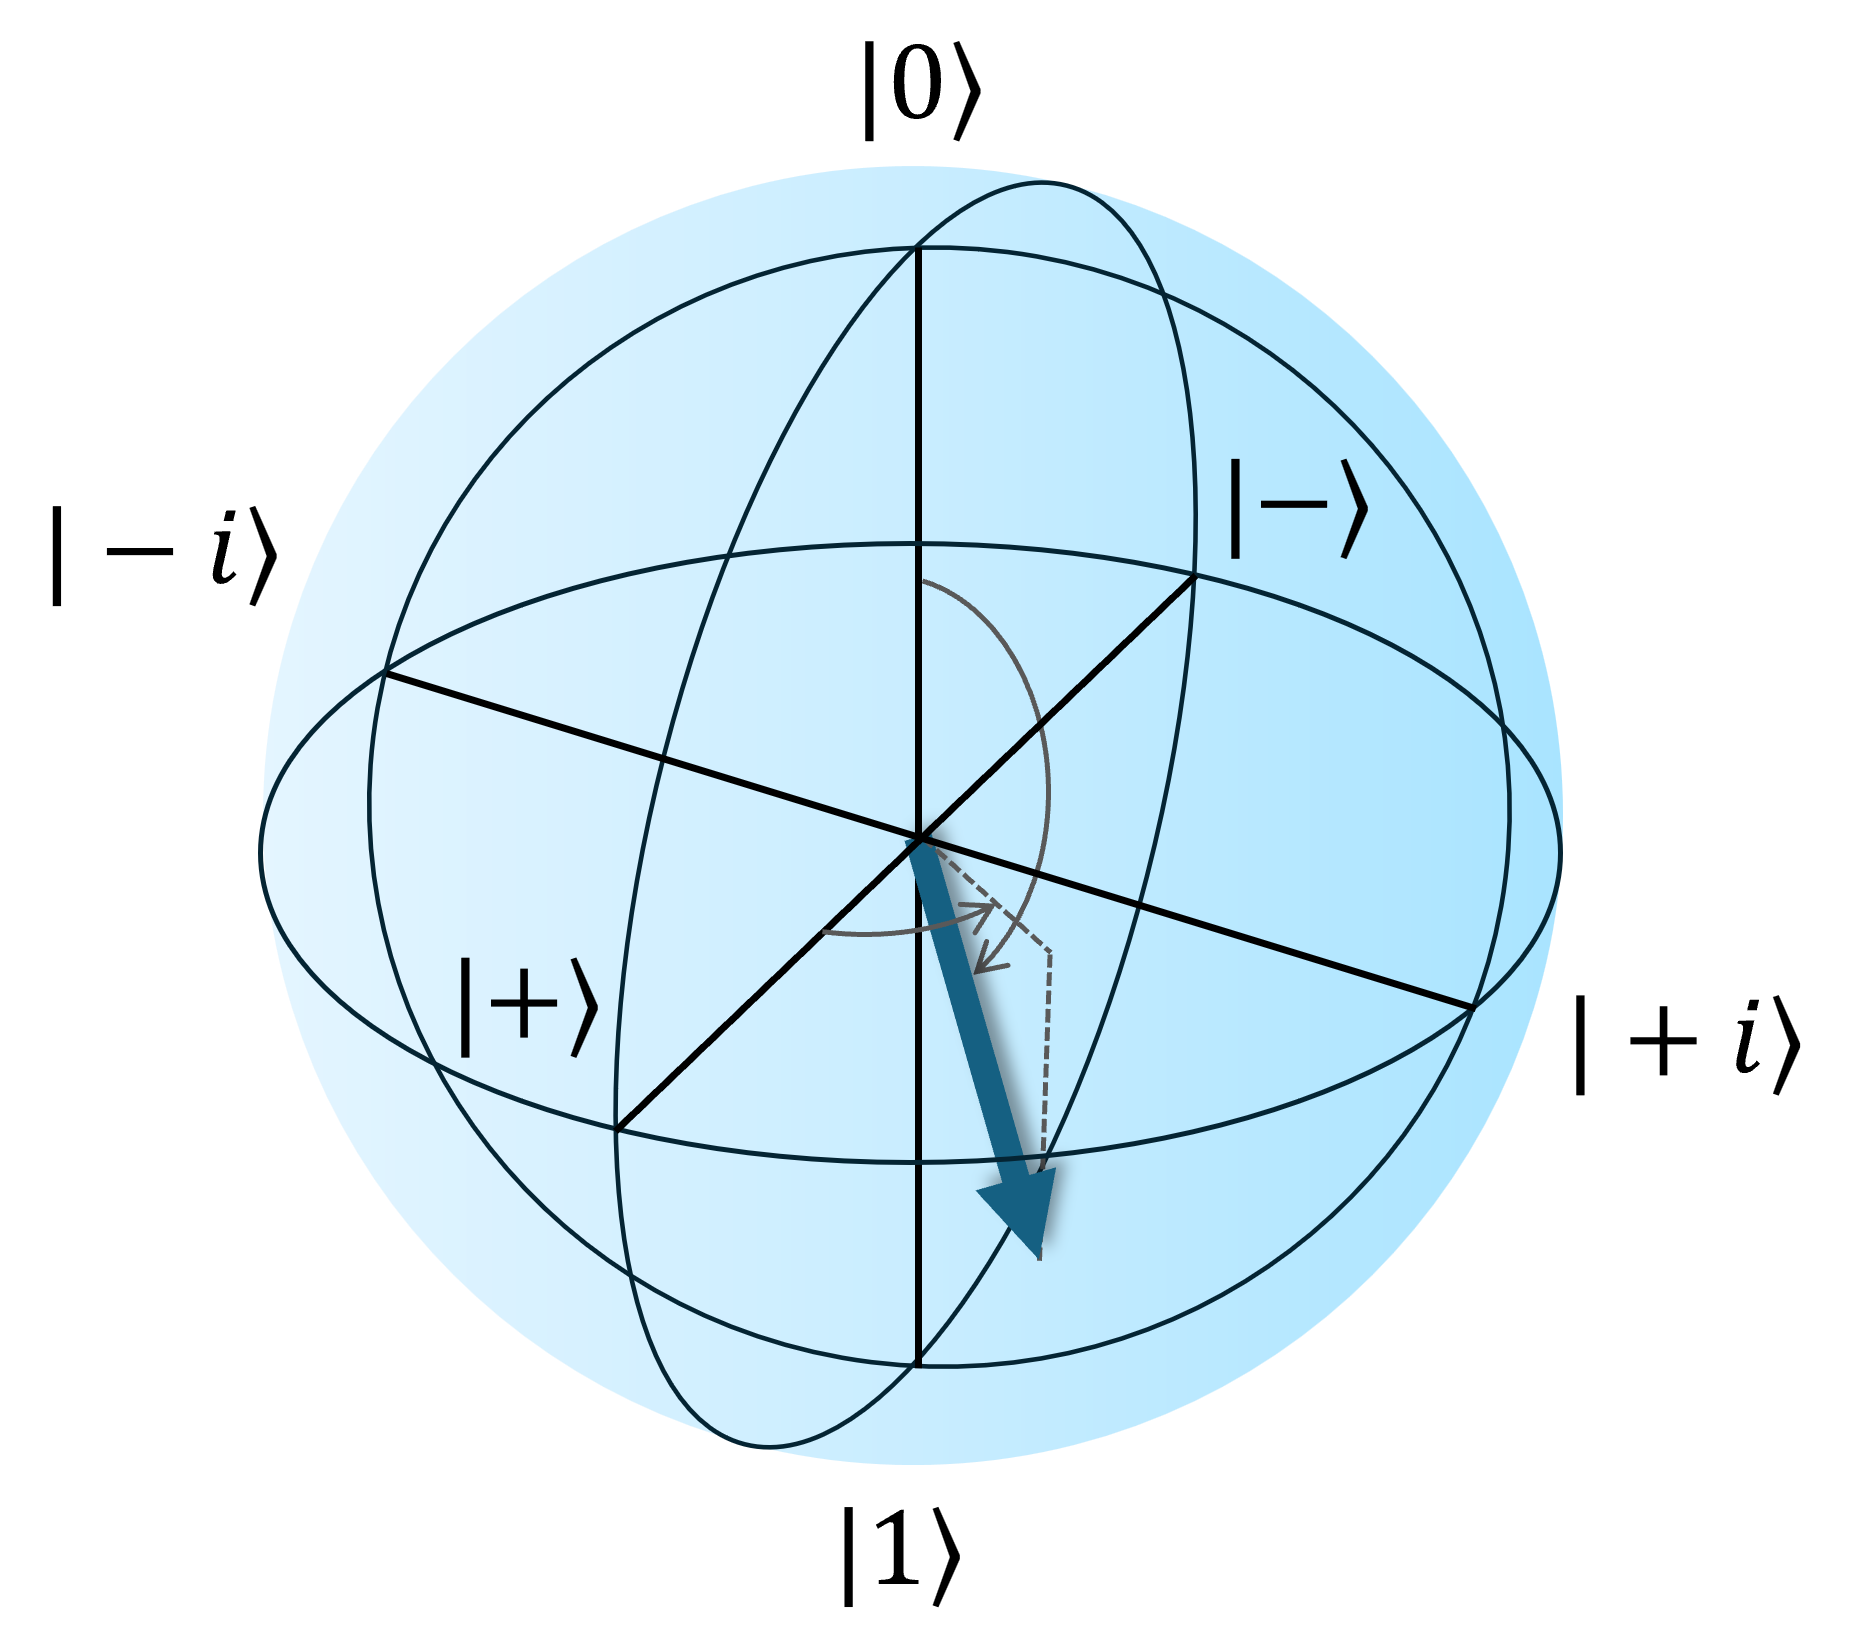
\includegraphics[width=0.22\linewidth]{images/PauliY_gate1.png}} \\[10pt]
            \hline
            \raisebox{-.5\height}{\parbox[c]{1em}{\centering Z}} & \raisebox{-.5\height}{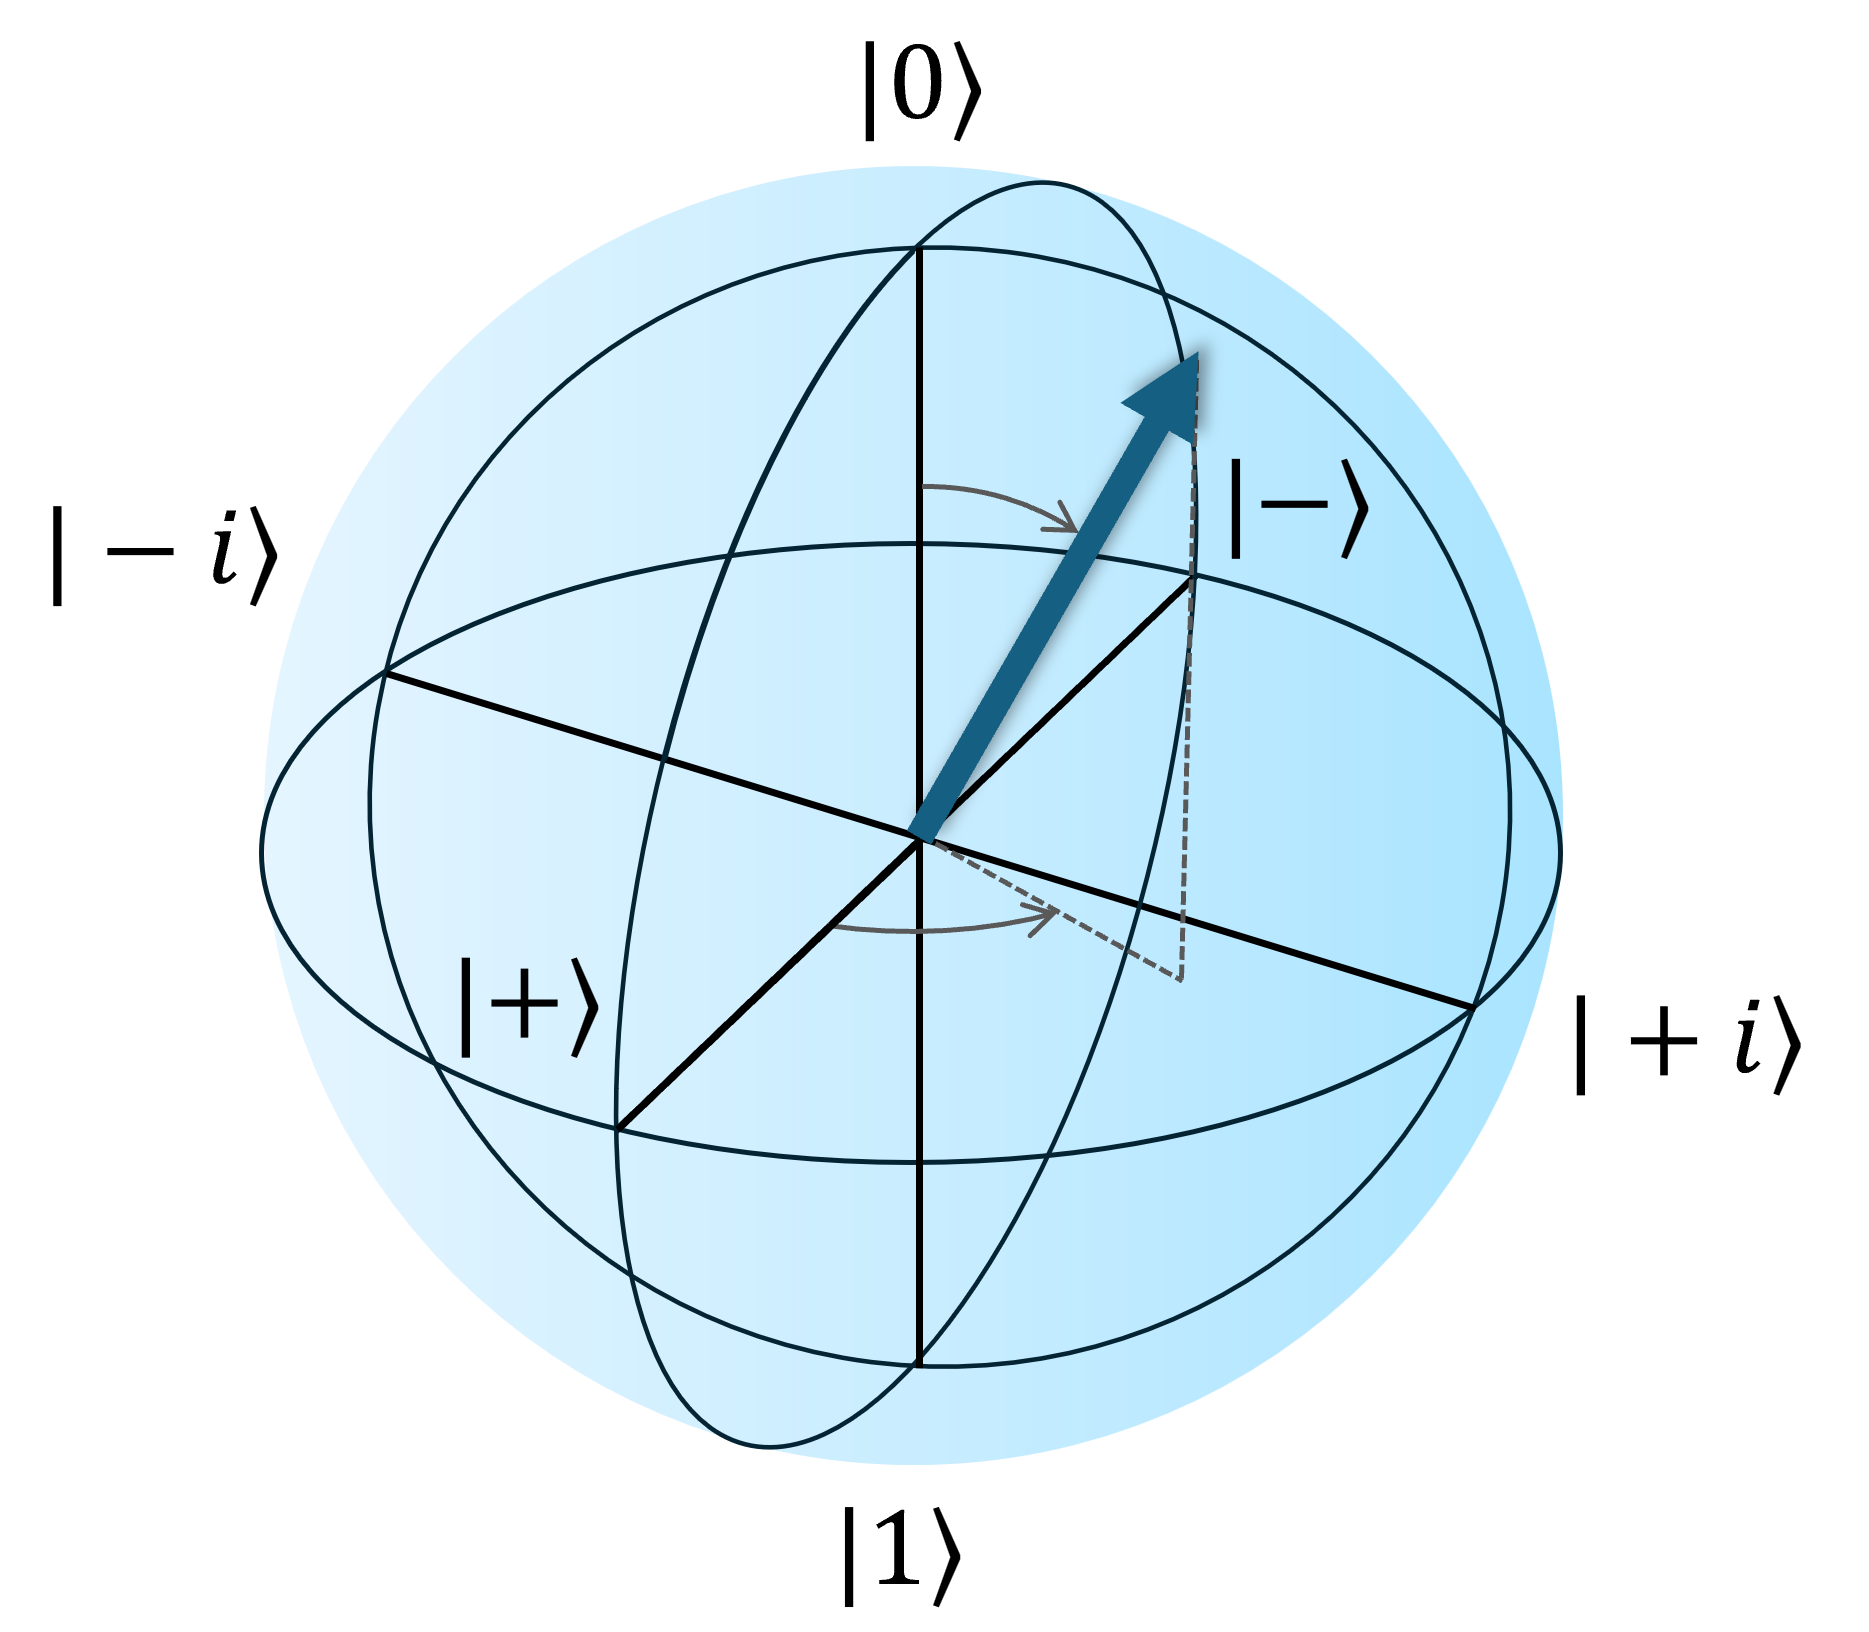
\includegraphics[width=0.22\linewidth]{images/PauliZ_gate0.png}} &
            \raisebox{-.5\height}{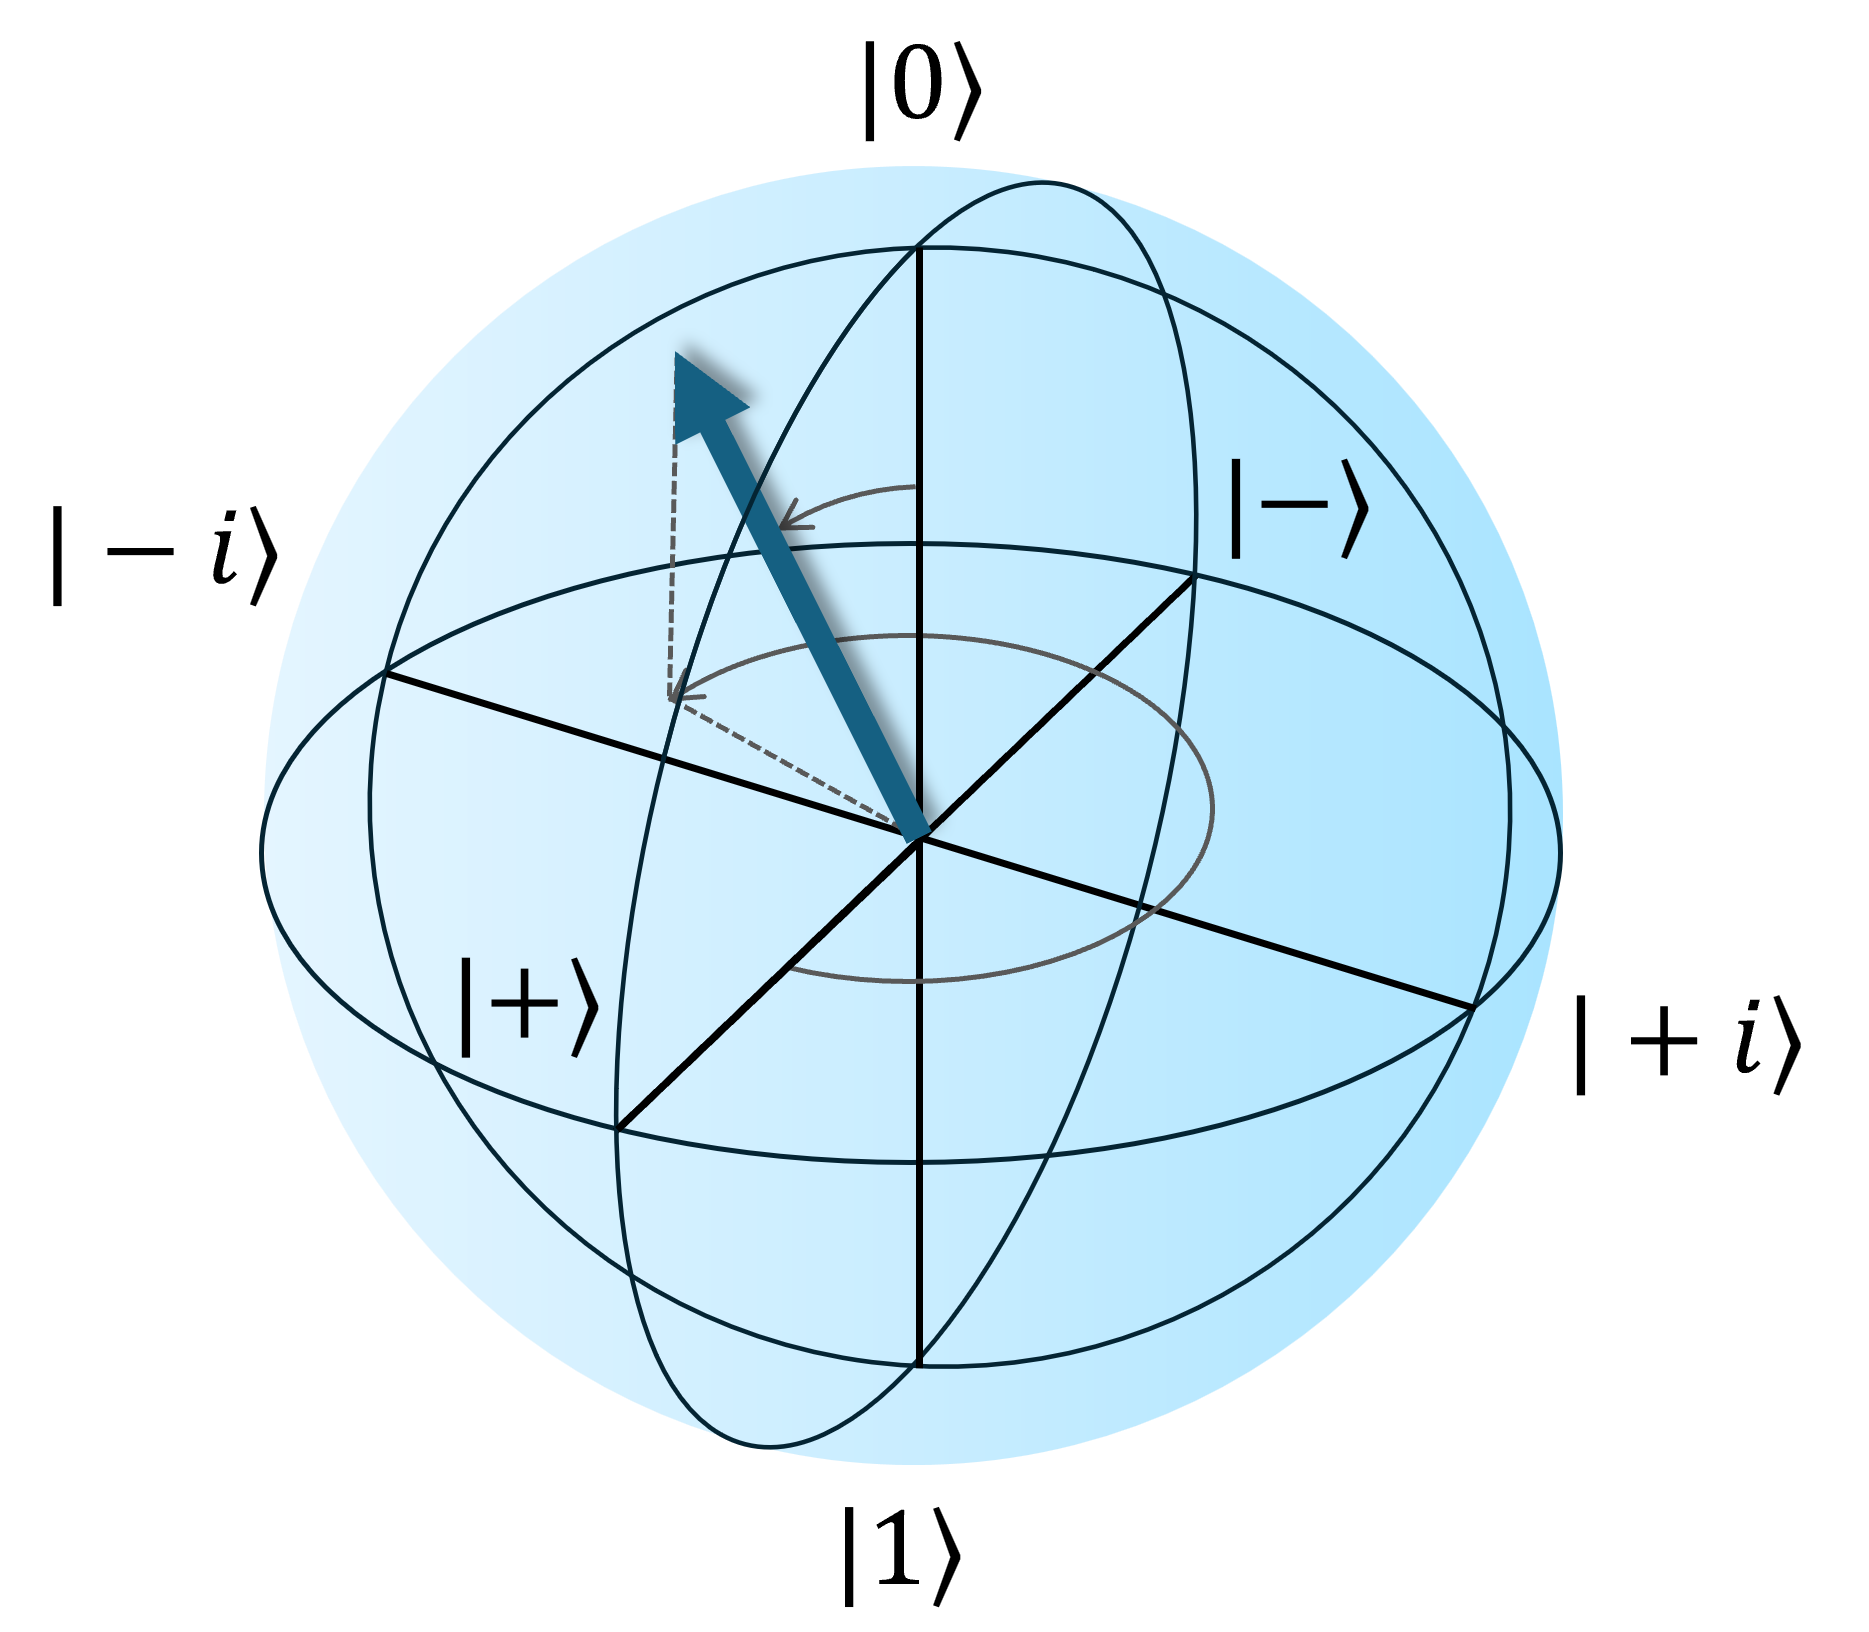
\includegraphics[width=0.22\linewidth]{images/PauliZ_gate1.png}} \\[10pt]
            \hline
        \end{tabular}
    \end{table}
    \pagebreak
    \item Hadamard-Gatter (H-Gatter): Ein Hadamard-Gatter erzeugt Superpositionen. Dies wird wie folgt dargestellt:
    $|0\rangle \rightarrow \frac{1}{\sqrt{2}}(|0\rangle + |1\rangle)$.\\
    Jedes Quantengatter ist umkehrbar. Das spezielle beim Hadamard-Gatter ist, dass es in den Ursprungszustand zurückführt:
    $\frac{1}{\sqrt{2}}(|0\rangle + |1\rangle) \rightarrow |0\rangle$ \cite{ct2020quantengatter}.

    \begin{table}[ht]
        \centering
        \caption{Hadamard-Gatter Darstellung}
        \label{tab:hadamard_gates}
        \begin{tabular}{|c|c|}
            \hline
            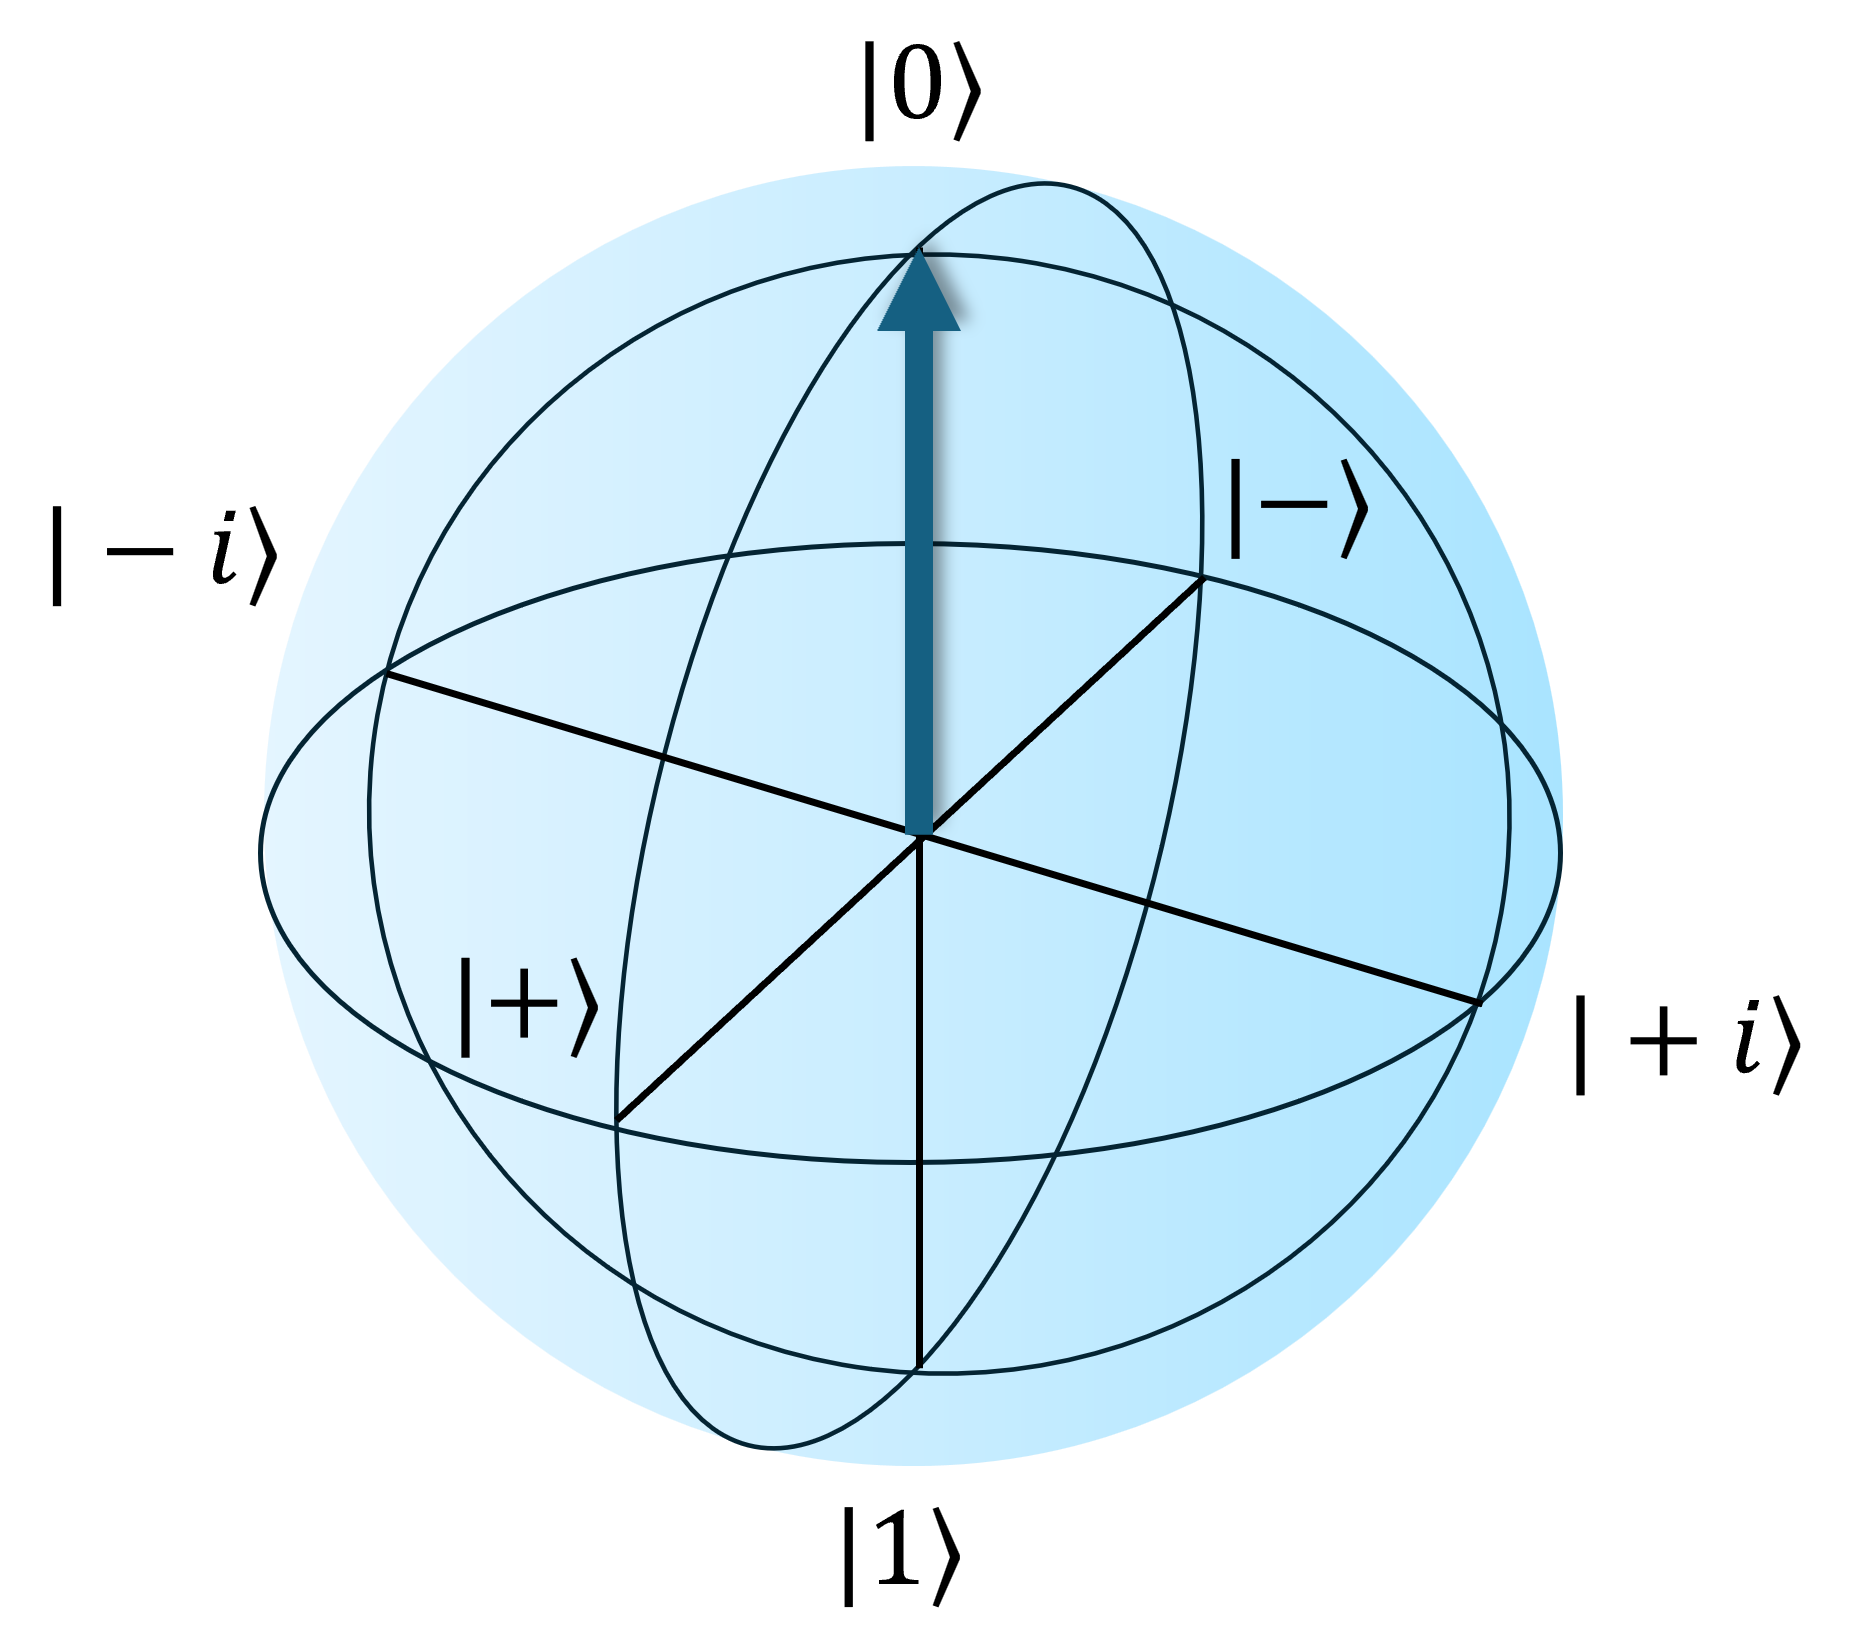
\includegraphics[width=0.3\linewidth]{images/Hadamard_gate0.png} &
            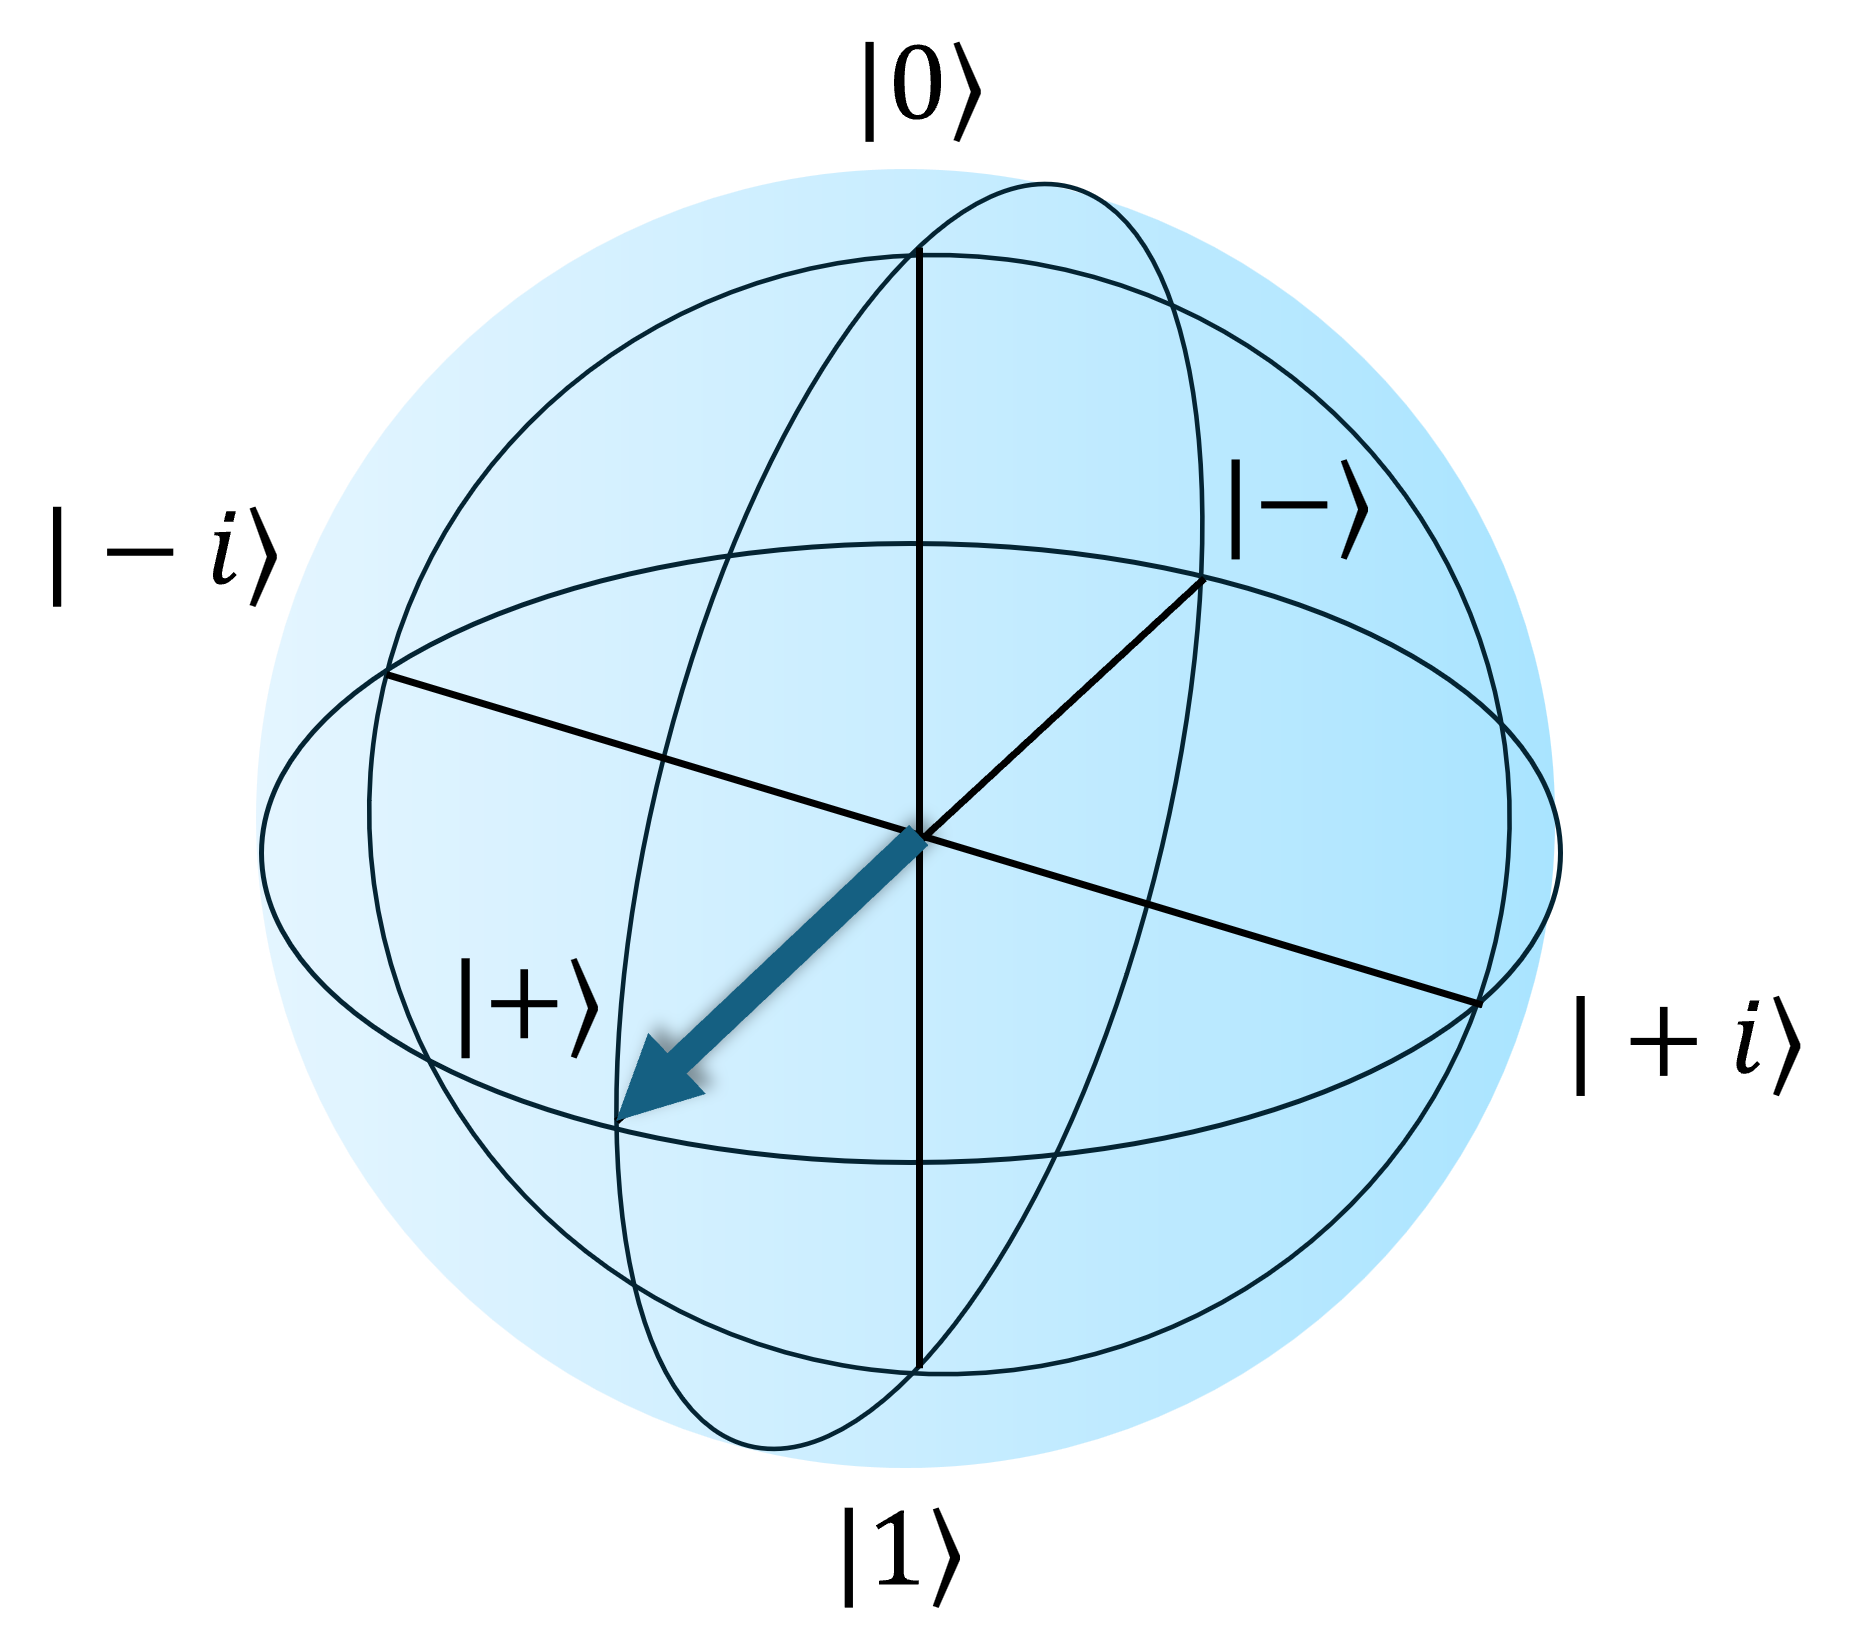
\includegraphics[width=0.3\linewidth]{images/Hadamard_gate1.png} \\
            \hline
        \end{tabular}
    \end{table}
    
    \item CNOT-Gatter: Ein CNOT-Gatter ist ein zwei-Qubit-Gatter, das den Zustand des zweiten Qubits ändert, wenn das erste Qubit im Zustand $|1\rangle$ ist \cite{ct2020quantengatter}.
    \begin{table}[ht]
        \centering
        \caption{CNOT-Gatter Darstellung}
        \label{tab:cnot_gates}
        \begin{tabular}{|c|c|}
            \hline
            \textbf{Qubit 1} & \textbf{Qubit 2} \\
            \hline
            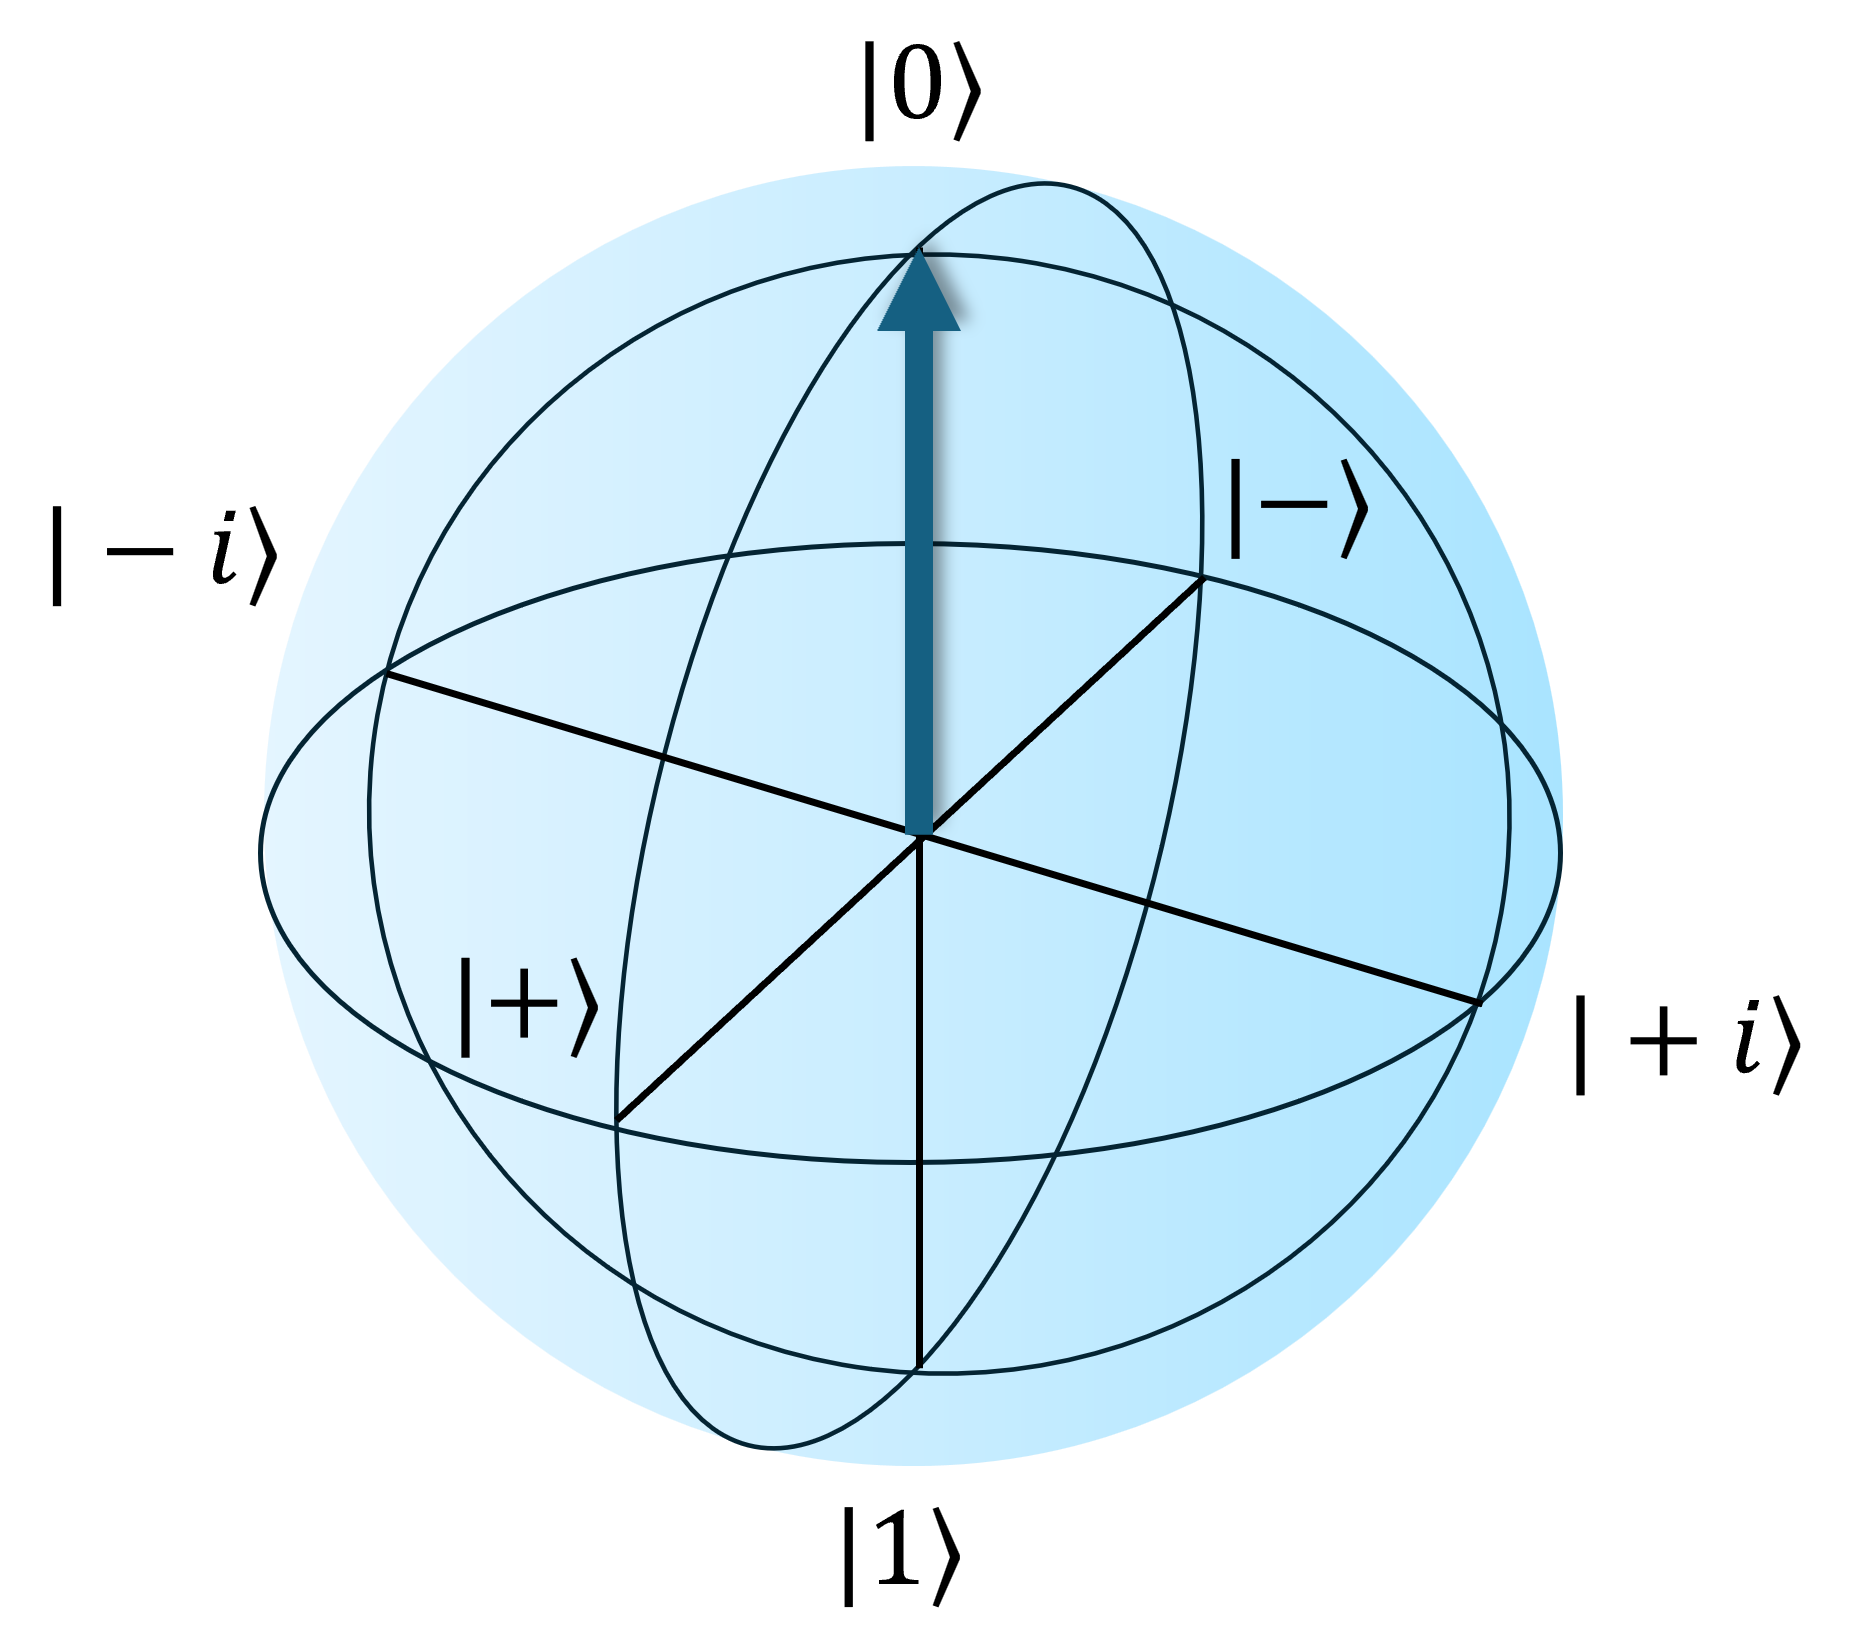
\includegraphics[width=0.3\linewidth]{images/Hadamard_gate0.png} &
            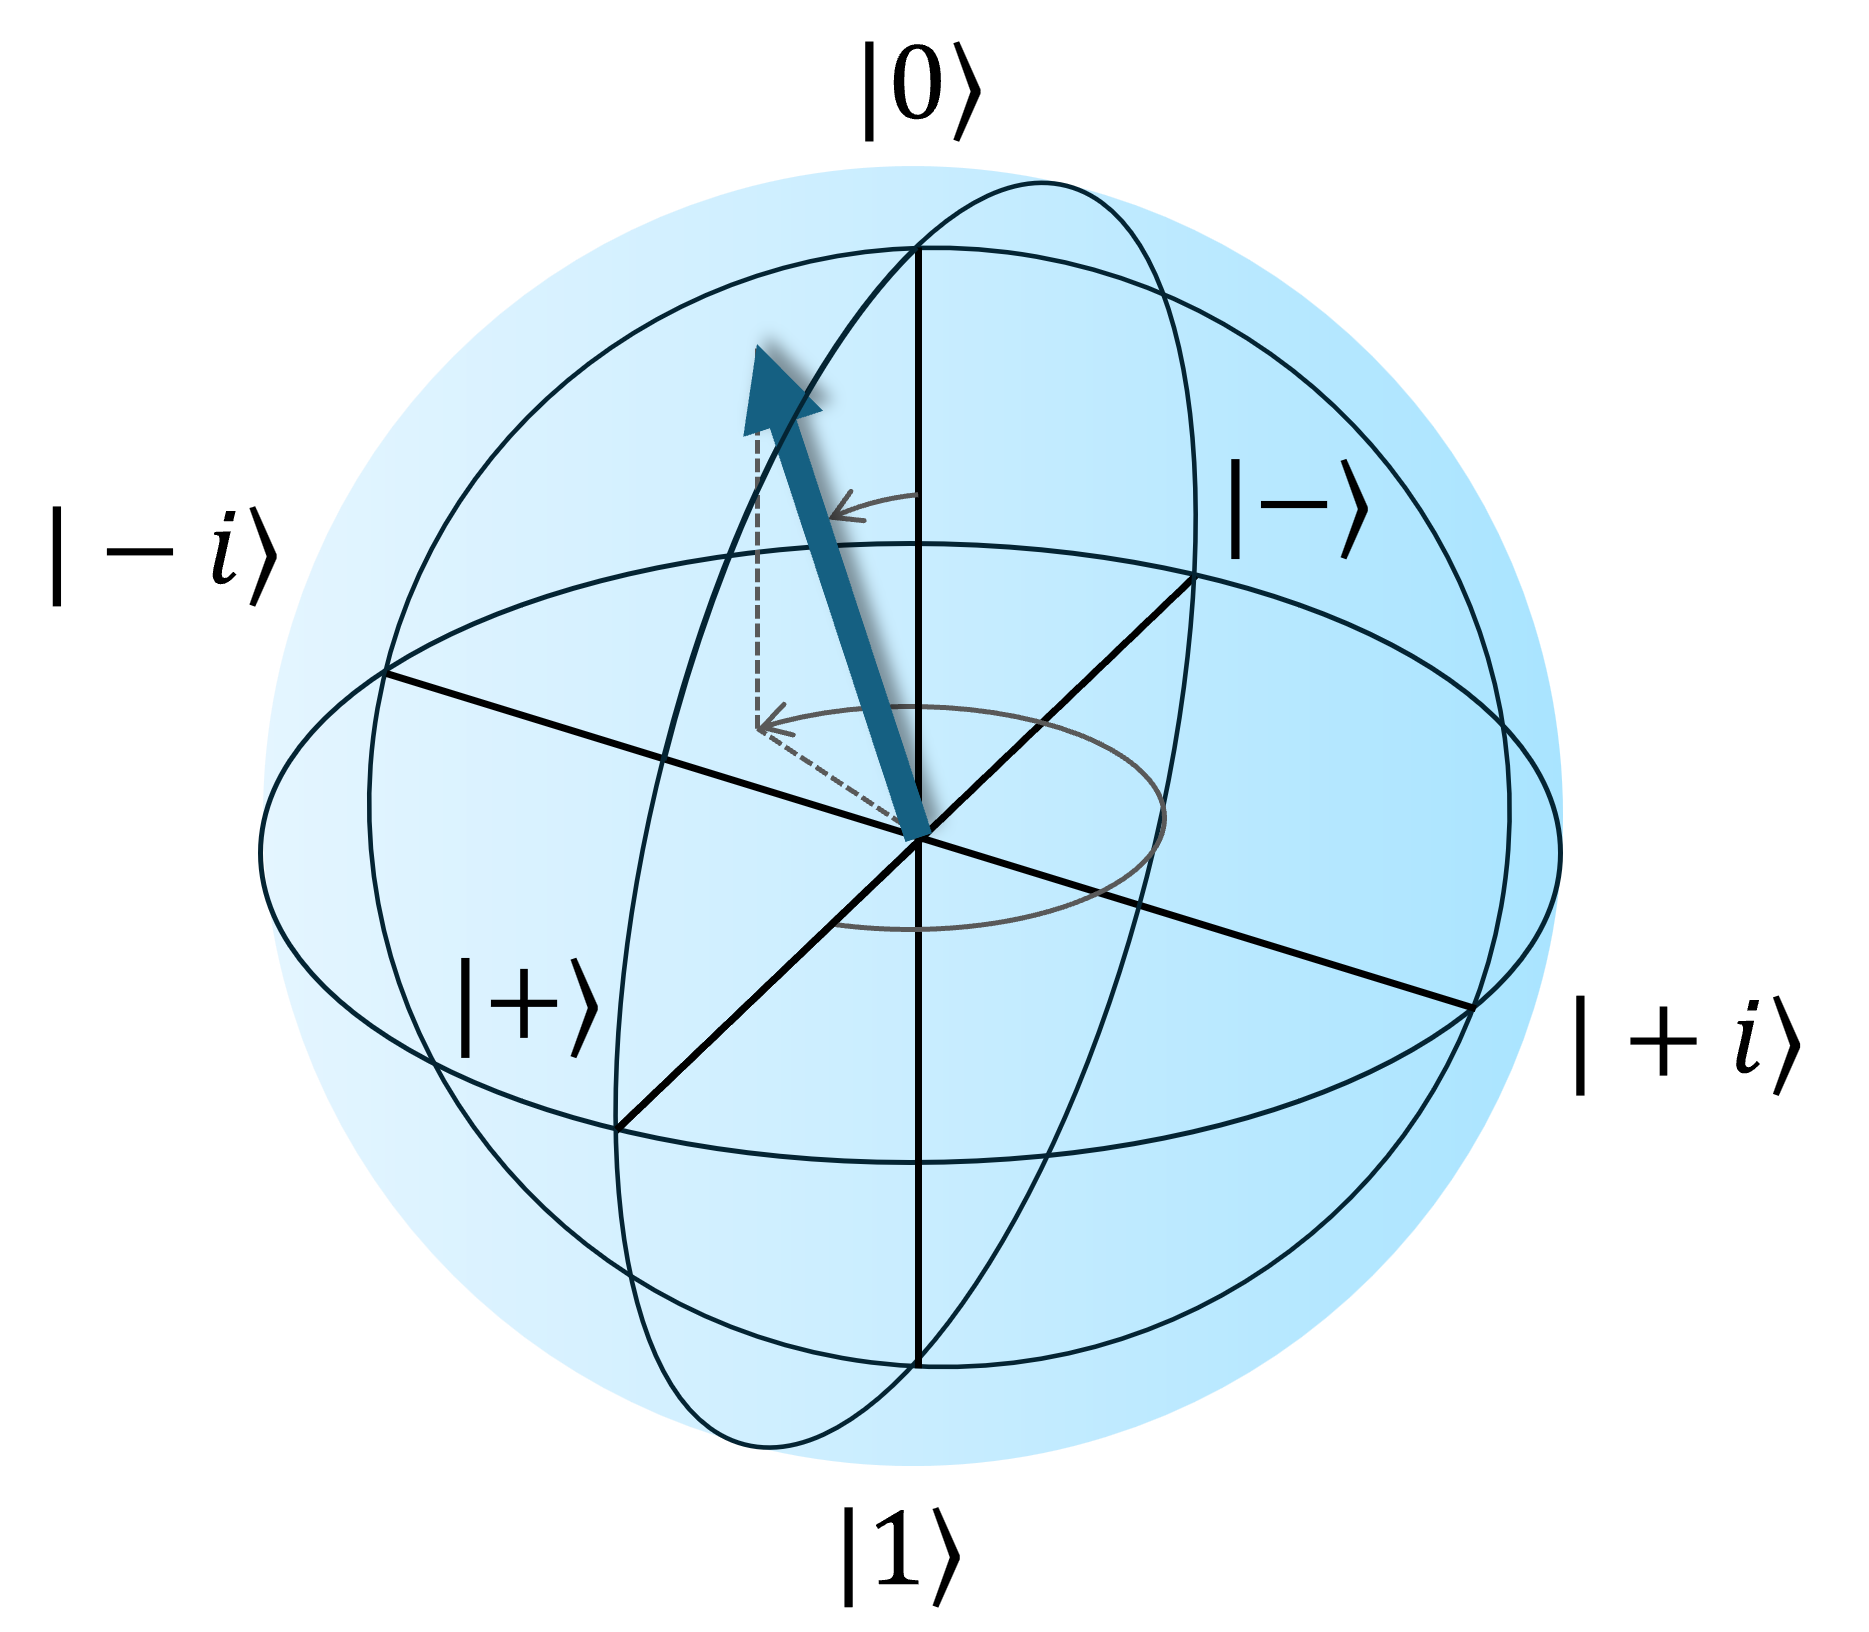
\includegraphics[width=0.3\linewidth]{images/PauliX_gate0.png} \\[5pt]
            \hline
            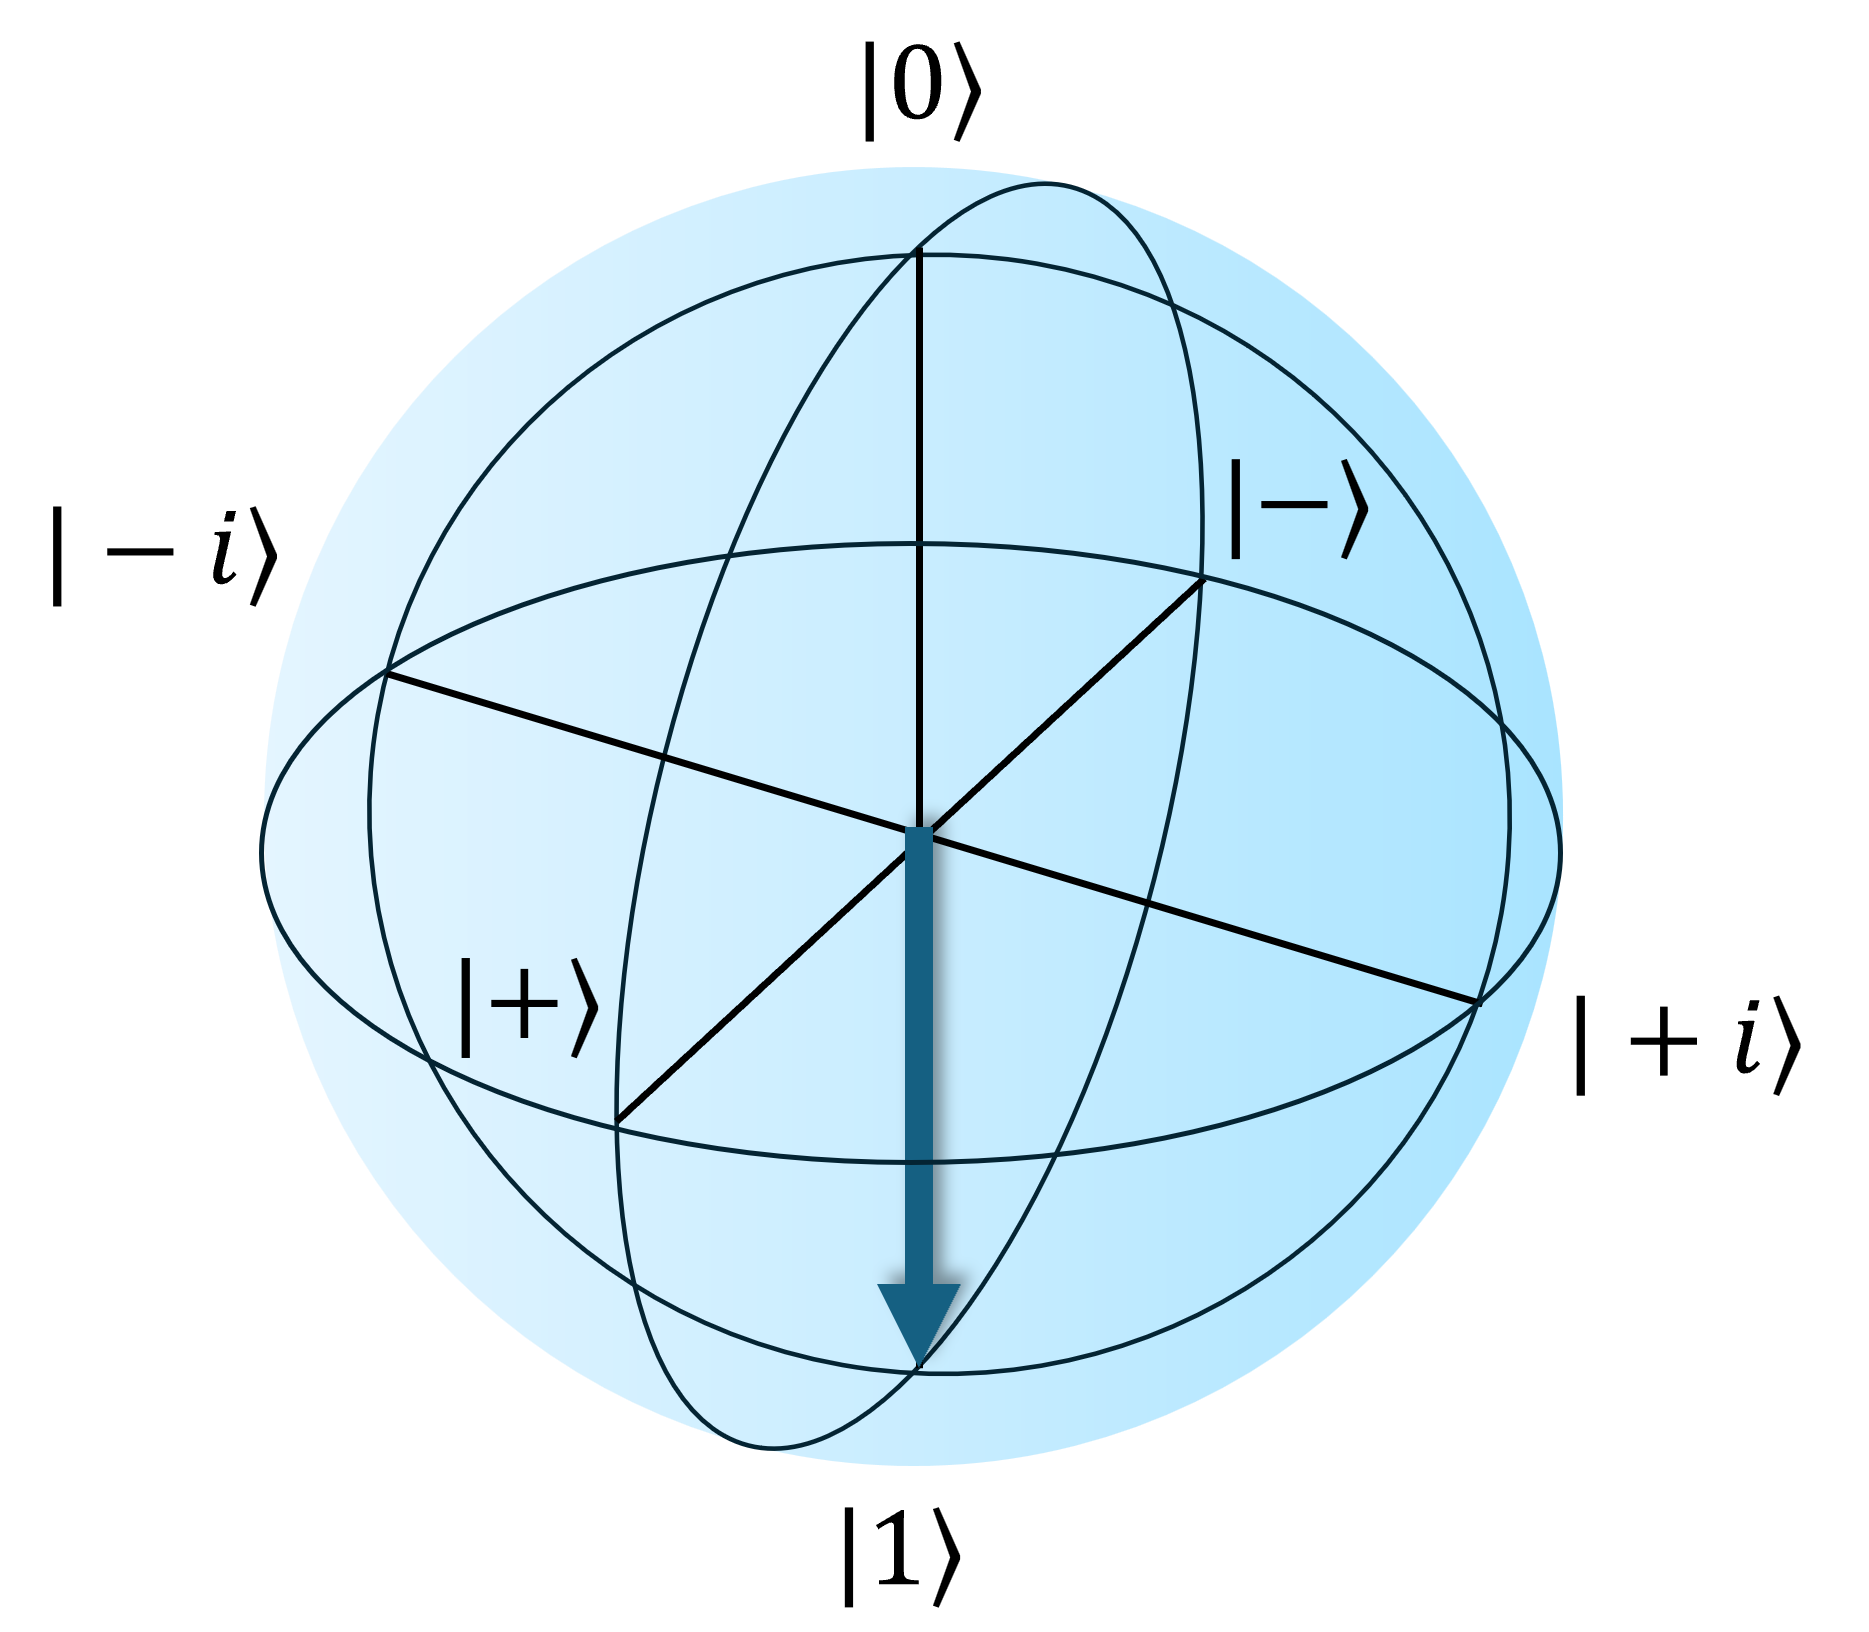
\includegraphics[width=0.3\linewidth]{images/gate_ket1.png} &
            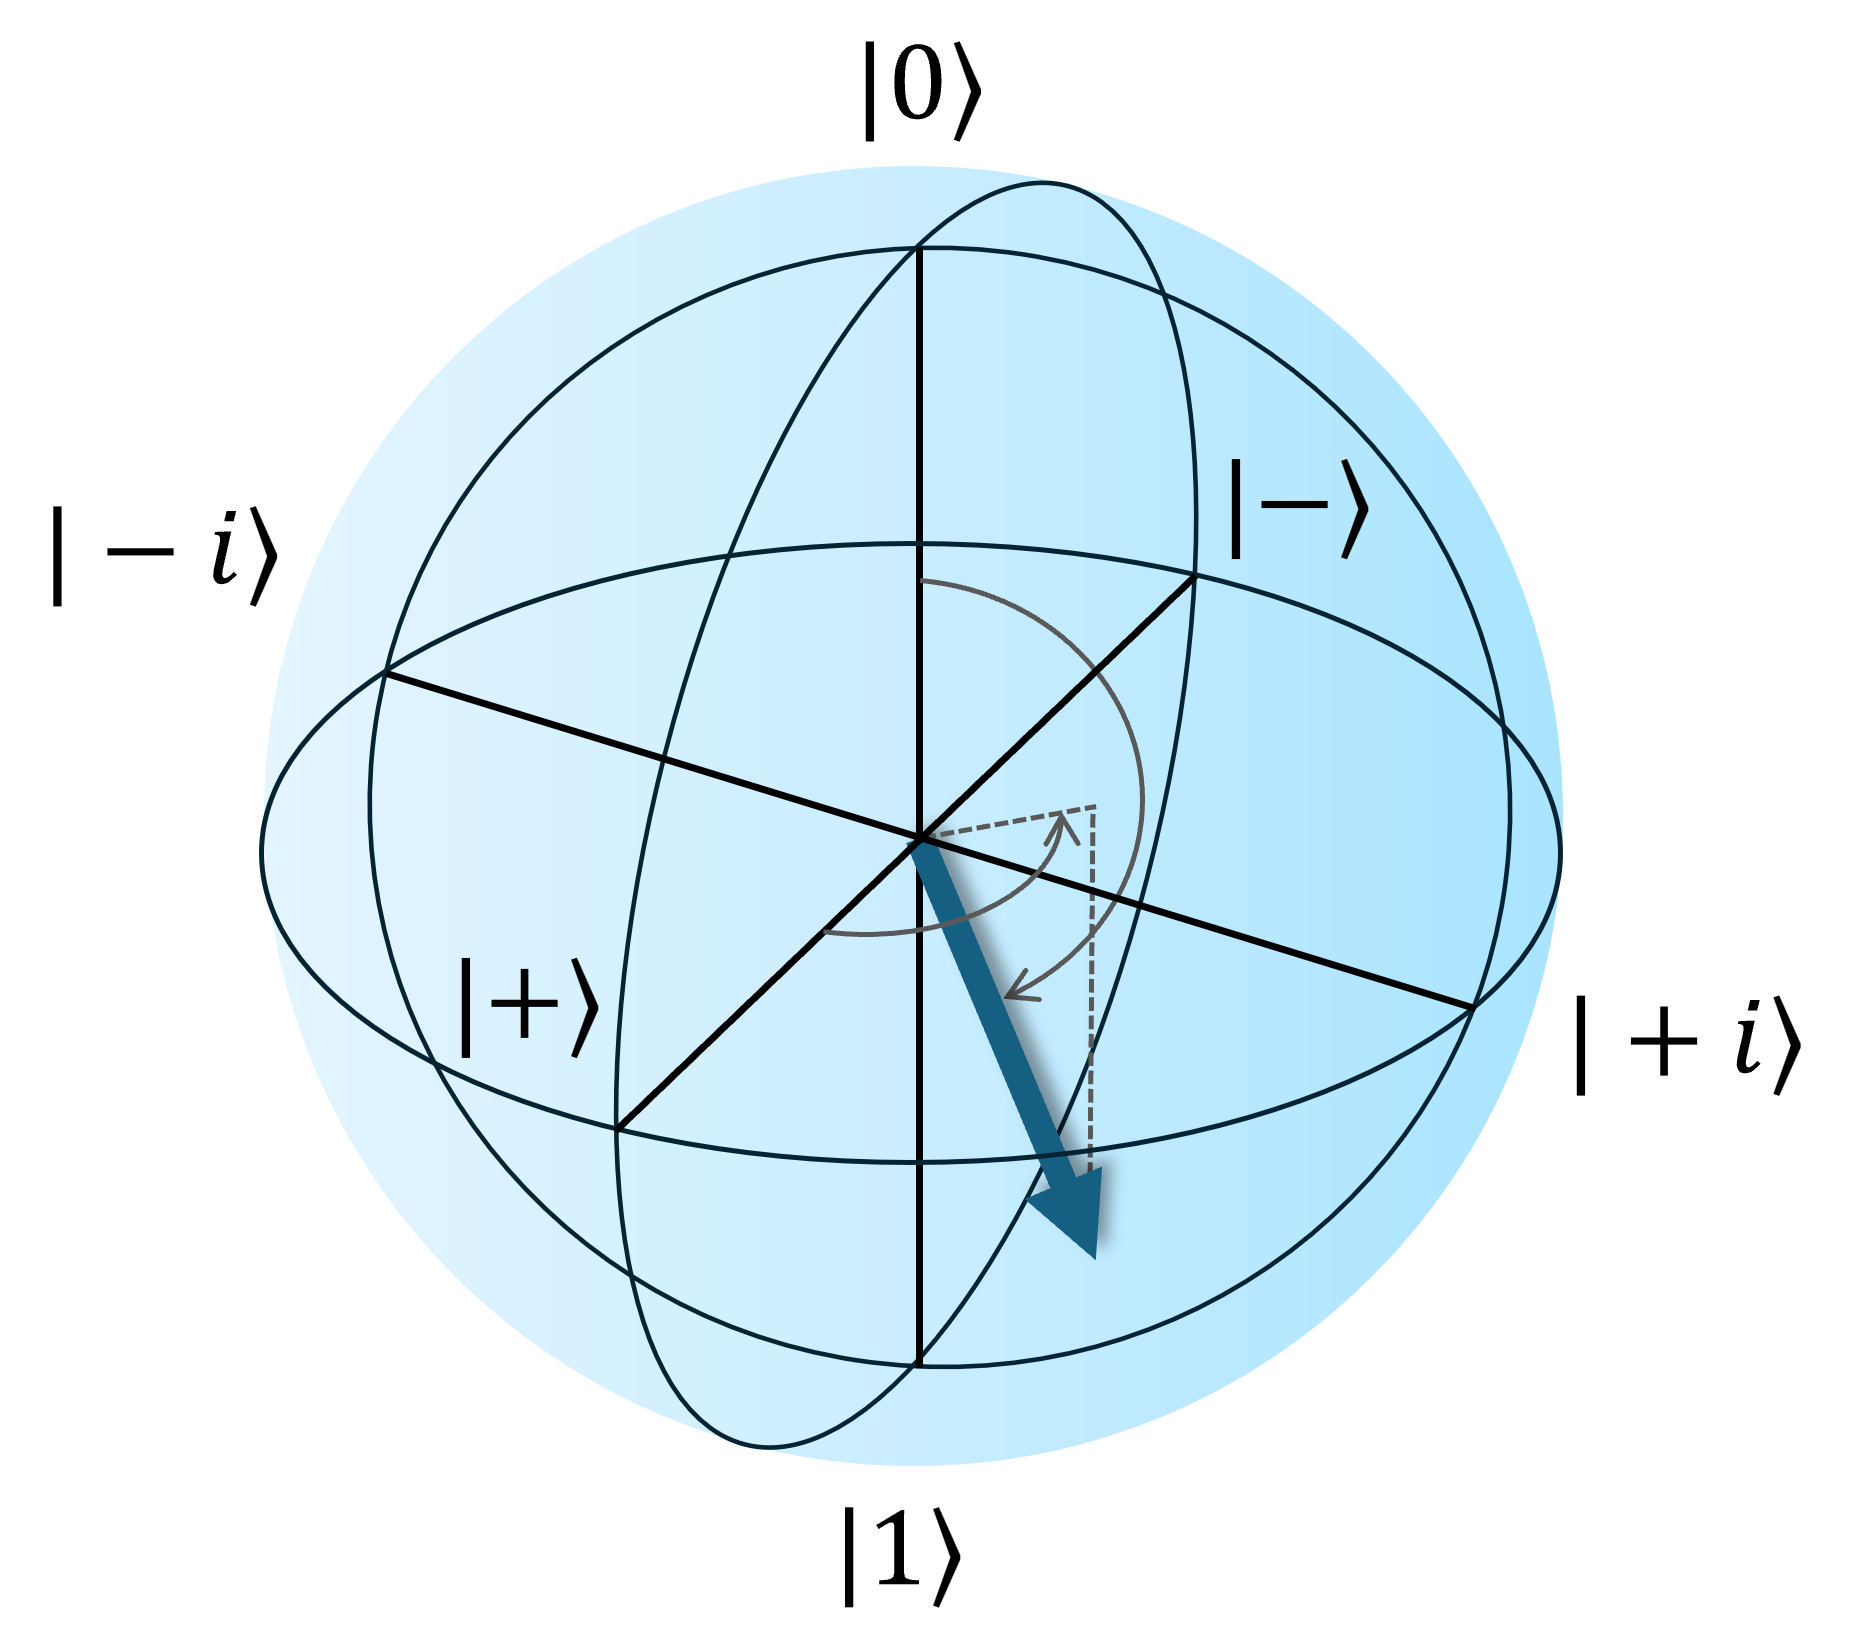
\includegraphics[width=0.3\linewidth]{images/PauliX_gate1.png} \\
            \hline
        \end{tabular}
    \end{table}
    \item Phasengatter: Das Phasengatter ändert die Phase eines Qubits ohne dessen Amplitude zu beeinflussen \cite{ct2020quantengatter}.
    \item CCNOT-Gatter (Toffoli-Gatter): Das CCNOT-Gatter ist ein Drei-Qubit-Gatter, das den Zustand des dritten Qubits ändert, wenn die ersten beiden Qubits im Zustand $|1\rangle$ sind \cite{bashiri2025quantencomputing}.
    \item SWAP-Gatter: Das SWAP-Gatter vertauscht die Zustände von zwei Qubits \cite{bashiri2025quantencomputing}.
    \item $R_k$-Gatter: Das $R_k$-Gatter rotiert den Zustand eines Qubits um einen Winkel von $\frac{2\pi}{2^k}$ um die Z-Achse der Bloch-Kugel \cite{bashiri2025quantencomputing}.
\end{itemize}

\newpage
\section{Rechengeschwindigkeit}
Quantencomputer haben das Potenzial, bestimmte Rechenprobleme, für die klassische Computer Jahre oder Jahrzehnte benötigen, in Sekunden oder Minuten zu lösen. 
Dies liegt an ihrer Fähigkeit, die Prinzipien der Quantenmechanik wie Superposition und Verschränkung zu nutzen, um Berechnungen parallel durchzuführen \cite{eth2023quantencomputer}.
\\
Während klassische Computer Informationen sequenziell verarbeiten, können Quantencomputer durch die gleichzeitige Verarbeitung vieler Zustände eine erhebliche Beschleunigung bei spezifischen Problemen erreichen. 
Ein Beispiel hierfür ist der Shor-Algorithmus (siehe Kapitel \ref{sec:Shor-Algorithmus}), der die Faktorisierung grosser Zahlen, ein nahezu exponentiell wachsendes Problem, in \hyperlink{polynomialtime}{Polynomzeit} ermöglicht \cite{bashiri2025quantencomputing}.
Die Abbildung \ref{fig:vergleich_polynom_exponentiel} zeigt einen Vergleich der Wachstumsraten.
\begin{figure}[ht]
    \centering
    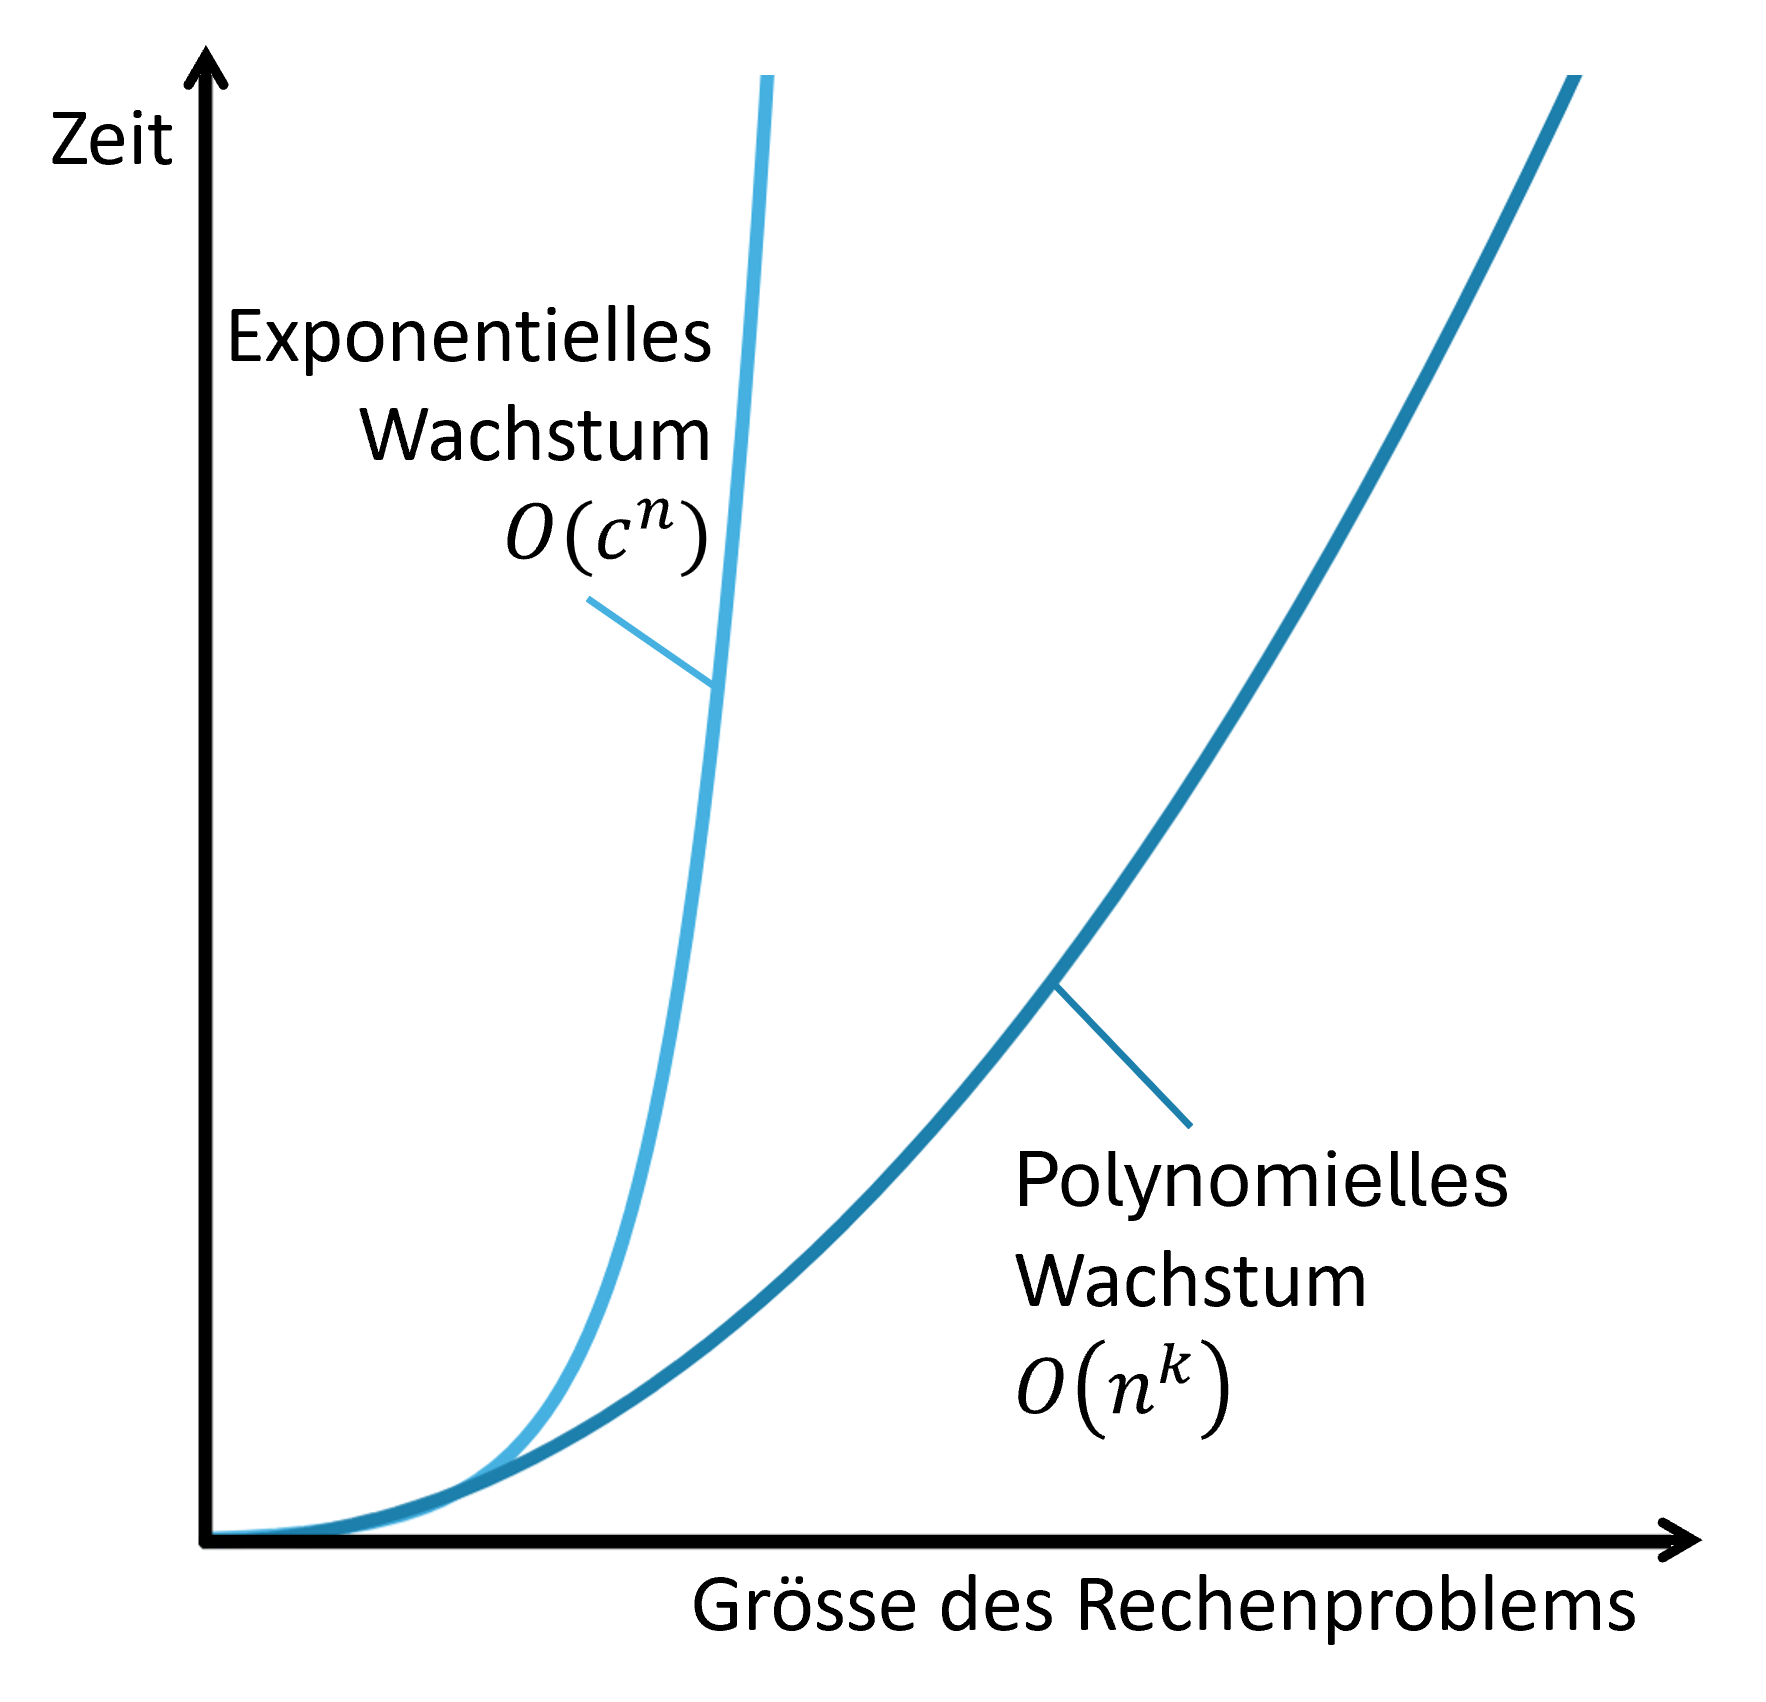
\includegraphics[width=0.4\linewidth]{images/Comparison_polynomiel_exponentiel.png}
    \caption{Vergleich Polynomielle und Exponentielle Wachstumsraten}
    \label{fig:vergleich_polynom_exponentiel}
\end{figure}\\
Ein weiterer bedeutender Algorithmus ist der Grover-Algorithmus, der für die Suche in unsortierten Datenbanken verwendet wird. 
Ein klassischer Algorithmus benötigt im Durchschnitt $\frac{N}{2}$ Schritte, um ein Element in einer unsortierten Datenbank mit $N$ Einträgen zu finden \cite{3blue1brownGrover}. 
Mit der \hypertarget{landau-notation-def}{Landau-Notation} wird dies ausgedrückt durch $O(N)$, $O$ steht hierbei für die Konstante und $N$ für die Eingangsgrösse \cite{landauNotation}.
Der Grover-Algorithmus hingegen reduziert die Anzahl der benötigten Schritte auf etwa $O(\sqrt{N})$ \cite{3blue1brownGrover}.
Die Abbildung \ref{fig:vergleich_linear_sqrt} zeigt einen Vergleich der Wachstumsraten.
\begin{figure}[ht]
    \centering
    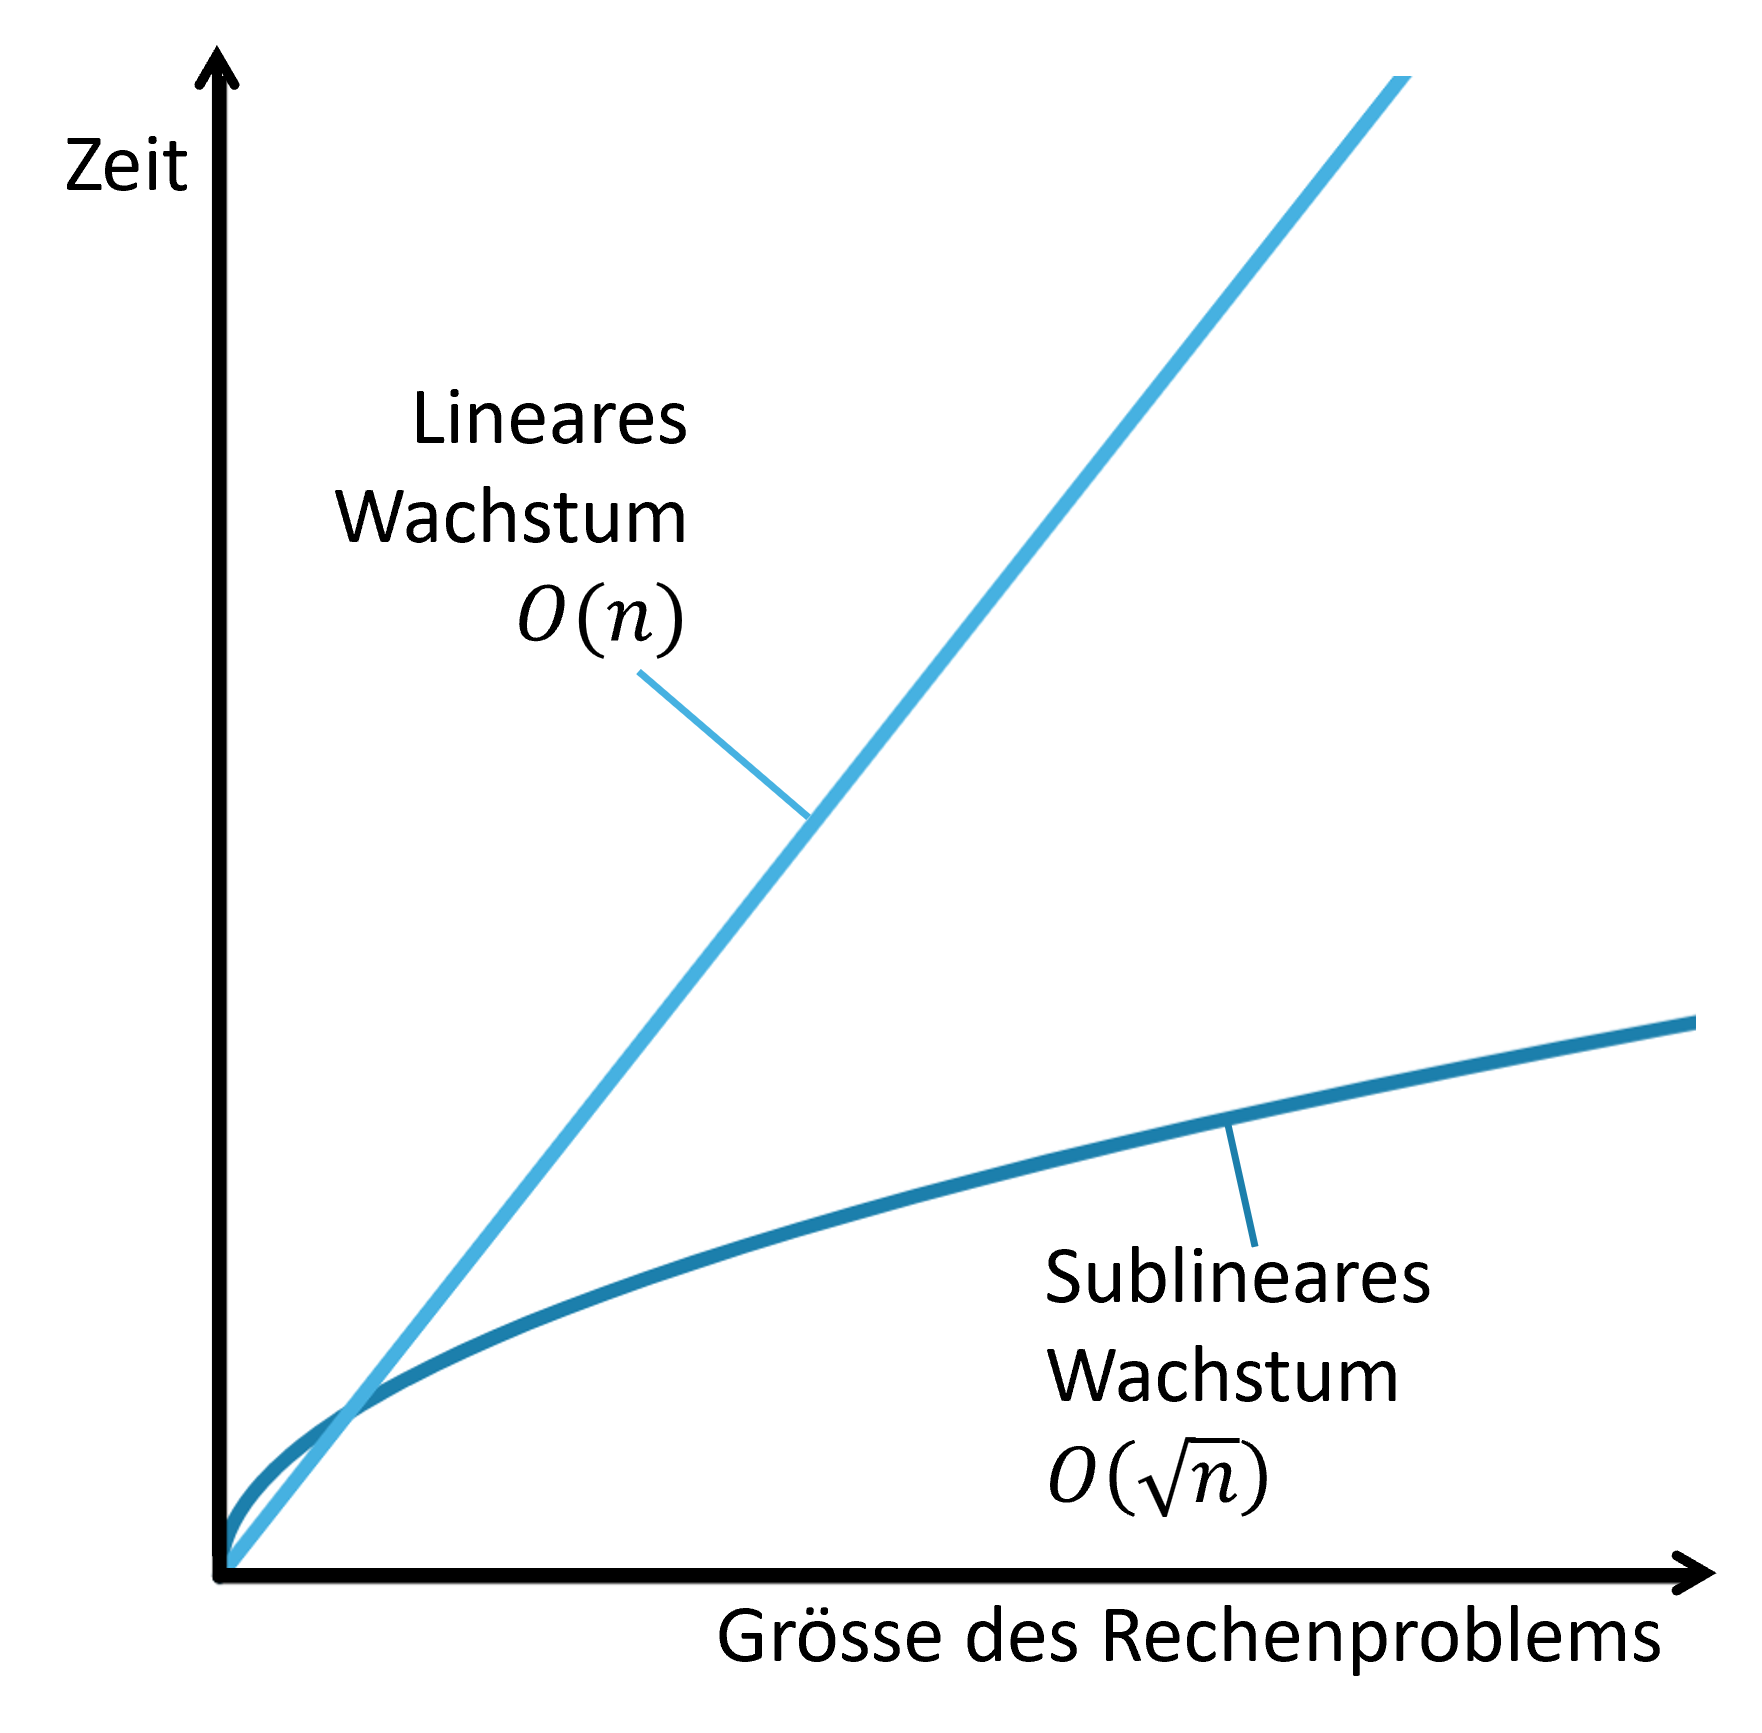
\includegraphics[width=0.4\linewidth]{images/Comparison_linear_sqrt.png}
    \caption{Vergleich Lineare und Sublineare Wachstumsraten}
    \label{fig:vergleich_linear_sqrt}
\end{figure}\\
Es ist jedoch wichtig zu betonen, dass Quantencomputer keine universelle Beschleunigung für alle Probleme bieten. 
Viele Probleme, die auf klassischen Computern exponentiell wachsen, können auch auf Quantencomputern noch nicht effizient gelöst werden.
Dazu wurden noch keine Algorithmen entwickelt.
\\
Klassische Computer können exponentiell wachsende Probleme nur schwer bewältigen. 
Quantenalgorithmen wie der Shor- und Grover-Algorithmus ermöglichen eine signifikante Reduktion der Rechenzeit \cite{eth2023quantencomputer}.

\newpage

\section{Aktueller Stand der Entwicklung}
%\subsection{Einsatzgebiete}
Der aktuelle Einsatz von Quantencomputern findet vor allem in Forschung und Entwicklung statt, insbesondere an Universitäten, in Forschungseinrichtungen und in industriellen Pilotprojekten \cite{eth2023quantencomputer}. 
Mögliche zukünftige Anwendungsfelder liegen unter anderem in Optimierungsproblemen, Materialforschung und spezifischen Simulationsaufgaben. 
Breit verfügbare, wirtschaftlich skalierbare Praxisanwendungen sind zum aktuellen Zeitpunkt jedoch weiterhin begrenzt \cite{weekly2025herausforderungen}.

\subsection{Herausforderungen}
Es gibt noch einige Herausforderungen bei der Entwicklung von Quantencomputern, die überwunden werden müssen, bevor sie weit verbreitet eingesetzt werden können.
Generell sind Qubits sehr anfällig für Störungen aus der Umwelt, wie thermisches Rauschen, elektromagnetische Felder oder Vibrationen, was zu Fehlern in Berechnungen führen kann.
Aktuell haben Quantencomputer nur eine begrenzte Anzahl von Qubits, was ihre Leistungsfähigkeit einschränkt. 
Es gibt verschiedene physikalische Realisierungen von Qubits, wobei jede Technologie eigene Herausforderungen in Bezug auf Stabilität, Skalierbarkeit und Fehleranfälligkeit mit sich bringt.
Supraleitende Qubits, wie sie bei den Quantencomputern von IBM (siehe Abbildung \ref{fig:ibm_quantum_one}) und Google zum Einsatz kommen, erfordern Temperaturen nahe dem absoluten Nullpunkt (-273,15 °C = 0K), was einen erheblichen technischen Aufwand bedeutet \cite{weekly2025herausforderungen}.
\begin{figure}[h!]
    \centering
    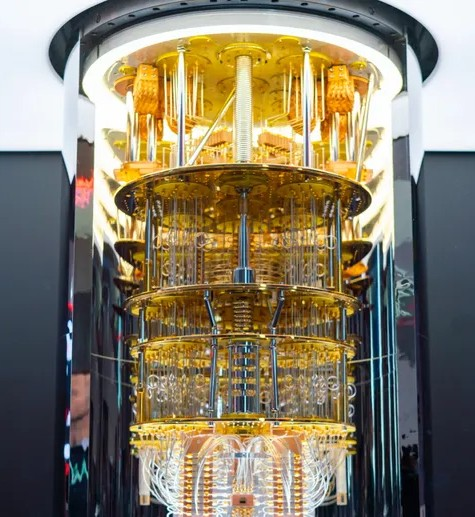
\includegraphics[width=0.25\linewidth]{images/IBM_quanutm_one.jpg}
    \caption{IBM Quantum System One \cite{spiegelIBMQuantum2021}.}
    \label{fig:ibm_quantum_one}
\end{figure}

\noindent
Einige Qubit-Technologien wie photonische Ansätze haben im Vergleich zu supraleitenden Systemen andere technische Randbedingungen, etwa beim Temperaturbedarf. 
Unabhängig von der Technologie bleiben jedoch zentrale Herausforderungen wie Fehleranfälligkeit, Skalierbarkeit und stabile Informationsübertragung bestehen \cite{weekly2025herausforderungen}.
\\
Um diese Herausforderungen zu bewältigen, werden verschiedene Ansätze verfolgt, darunter die Entwicklung von Quantenfehlerkorrekturmethoden und die Erforschung neuer Materialien für Qubits. 
Für ein logisches Qubit werden viele physikalische Qubits benötigt, um Fehler zu korrigieren.
Bis zum Jahr 2023 ging man davon aus, dass für ein logisches Qubit etwa 1000 bis 10'000 physikalische Qubits benötigt werden. 
Dann konnte ein Forschungsteam aus den USA einen fehlerkorrigierten Quantenalgorithmus auf 48 logischen Qubits ausführen \cite{spektrum2023quantenfehlerkorrektur}.
\pagebreak
\subsection{Dauer bis Marktreife}
Q-Day ist ein Begriff, der den Zeitpunkt beschreibt, an dem Quantencomputer in der Lage sein werden, 
praktische Probleme zu lösen, die für klassische Computer in akzeptabler Zeit unlösbar sind. 
\\
Gemäss der Roadmap der Quantenabteilung von IBM soll bis 2029 ein erster fehlertoleranter Quantencomputer mit 200 logischen Qubits präsentiert werden. 
Bis 2033 sollen es dann 2000 logische Qubits sein \cite{ct2025verschluesselung}. 
Um eine RSA-Verschlüsselung zu brechen, braucht es jedoch etwa 4000 logische Qubits \cite{qday2030}.
\\
Das deutsche Bundesamt für Sicherheit in der Informationstechnik (BSI) hält 
einen Zeitpunkt in 10--16 Jahren (Stand 2025) realistisch, bis ein Quantencomputer mit 2000 logischen Qubits veröffentlicht wird \cite{ct2025verschluesselung}.
Je nach technischer Annahme und Bewertungsgrundlage variieren Prognosen zum Q-Day jedoch deutlich.
Selbst Expertinnen und Experten sind sich daher uneinig, wann Quantencomputer marktreif sein werden.
\\
Gemäss dem BSI dürfte es sich für die meisten Firmen jedoch nicht lohnen, einen Quantencomputer mit mehr als 2000 logischen Qubits zu entwickeln, 
da diese Anzahl von logischen Qubits für Anwendungen in der Industrie oder Forschung ausreicht \cite{ct2025verschluesselung}.

